\documentclass[11pt]{article}

\usepackage[utf8]{inputenc}
\usepackage[T1]{fontenc}
\usepackage{amsmath,amssymb,amsthm}
\usepackage{mathtools}
\usepackage{algorithm}
\usepackage{algpseudocode}
\usepackage{booktabs}
\usepackage{graphicx}
\usepackage{hyperref}
\usepackage{xcolor}
\usepackage{listings}
\usepackage[margin=1in]{geometry}
\usepackage{enumitem}
\usepackage{tikz}
\usetikzlibrary{arrows.meta,positioning,shapes.geometric,fit,calc,cd}
\usepackage{multirow}
\usepackage{caption}
\usepackage{subcaption}

\newtheorem{theorem}{Theorem}
\newtheorem{lemma}[theorem]{Lemma}
\newtheorem{definition}[theorem]{Definition}
\newtheorem{proposition}[theorem]{Proposition}
\newtheorem{corollary}[theorem]{Corollary}
\newtheorem{remark}[theorem]{Remark}
\newtheorem{example}[theorem]{Example}

\newcommand{\Set}{\mathbf{Set}}
\newcommand{\Pow}{\mathcal{P}}
\newcommand{\Fair}{\ensuremath{\mathrm{Fair}}}
\newcommand{\Act}{\ensuremath{\mathrm{Act}}}
\newcommand{\AP}{\ensuremath{\mathrm{AP}}}
\newcommand{\WF}{\ensuremath{\mathrm{WF}}}
\newcommand{\SF}{\ensuremath{\mathrm{SF}}}
\newcommand{\TFair}{$T$-Fair}
\newcommand{\CoaCert}{\textsc{CoaCert-TLA}}
\newcommand{\TLAplus}{TLA\textsuperscript{+}}
\newcommand{\naturals}{\mathbb{N}}
\newcommand{\reals}{\mathbb{R}}
\newcommand{\diam}{\ensuremath{\mathrm{diam}}}
\newcommand{\FPR}{\ensuremath{\mathrm{FPR}}}
\newcommand{\Streett}{\ensuremath{\mathrm{Streett}}}

\lstset{
  basicstyle=\ttfamily\small,
  keywordstyle=\bfseries\color{blue!70!black},
  commentstyle=\itshape\color{gray},
  stringstyle=\color{red!60!black},
  frame=single,
  breaklines=true,
  columns=flexible,
}

\title{\CoaCert{}: Witness-Certified Coalgebraic Compression\\for Finite-Domain \TLAplus{} Model Checking}

\date{}

\begin{document}

\maketitle

%% ============================================================
%% ABSTRACT
%% ============================================================
\begin{abstract}
We present \CoaCert{}, a tool that compresses \TLAplus{} state spaces via
coalgebraic bisimulation quotienting and emits Merkle-hashed witnesses
enabling independent, third-party verification of the reduction's correctness.
The core theoretical contribution is a new endofunctor
$F(X) = \Pow(\AP) \times \Pow(X)^{\Act} \times \Fair(X)$
on the category $\Set$ whose coalgebra morphisms are precisely the
stuttering bisimulations respecting weak and strong fairness constraints
native to \TLAplus{}.
We establish a \emph{\TFair{} coherence theorem}---a distributive law
$\delta : T \circ \Fair \Rightarrow \Fair \circ T$ between the
stutter-closure monad~$T$ of Beohar and K\"upper and the fairness component---and
provide a full constructive proof by exhaustion over saturation conditions.
This coherence is both necessary and sufficient for $F$-bisimulations to
preserve Streett acceptance conditions, enabling liveness preservation
under weak and strong fairness.
By instantiating the Barlocco--Kupke--Rot categorical learning framework
for this functor, \CoaCert{} automatically computes minimal bisimulation
quotients via $L^*$-style active learning with
$O(n^2 k)$ membership queries.
We prove W-method completeness for bounded conformance testing at
depth $k = \diam(H) + (m - n + 1)$, establishing that automatic
conformance depth suffices for soundness.
The emitted Merkle-hashed witness binds every equivalence class to its
representative and every quotient transition to its original-system witnesses,
with Bloom-filter-backed compact representations whose false positive rate
is bounded by $(1 - e^{-kn/m})^k$; we prove a verification soundness
theorem relating the Bloom filter FPR to overall witness reliability.
On six standard distributed protocol benchmarks---Two-Phase Commit, Paxos,
Peterson's mutual exclusion, Leader Election, Token Ring, and Dining
Philosophers---\CoaCert{} achieves compression ratios from
$4\times$ to $50\times$ while preserving all stuttering-invariant
CTL$^*$$\setminus$X properties and liveness under fairness.
Comparison against a Paige--Tarjan partition-refinement baseline shows
that coalgebraic learning achieves comparable or better quotients while
additionally producing certified witnesses.
Witness verification runs in seconds, requires no access to the original
specification, and provides hash-based integrity and auditability.
The implementation comprises approximately 53{,}000 lines of Python
across 15~modules with a type-hardened verifier and independent cross-checker.
\end{abstract}

%% ============================================================
%% 1. INTRODUCTION
%% ============================================================
\section{Introduction}
\label{sec:intro}

The state explosion problem remains the central barrier to practical model
checking of distributed protocols specified in \TLAplus{}~\cite{Lamport02}.
TLC, Lamport's explicit-state checker~\cite{TLC}, exhaustively enumerates
every reachable state; for Two-Phase Commit with seven participants or
Paxos with three acceptors, this reaches hundreds of thousands to millions
of states.
Apalache's symbolic approach~\cite{Apalache} trades enumeration for SMT
encoding but encounters solver limits on the same protocols.
Critically, neither tool produces any independently inspectable
artifact---a user must trust the tool's implementation, its runtime, and the
machine it ran on.

The absence of certificates is not merely an aesthetic concern.
In safety-critical settings---aerospace control protocols, financial
settlement systems, medical device firmware---regulatory bodies increasingly
demand evidence beyond ``the tool reported success.''
Certified model checking~\cite{Namjoshi01} addresses this by requiring the
checker to emit a proof certificate that a lightweight verifier can
independently validate.
However, existing certified approaches target specific logics (CTL, LTL)
and specific algorithms (BDD-based symbolic checking), and none address
state-space compression with fairness preservation.

\CoaCert{} addresses both problems simultaneously.
The key insight is that Lamport's \emph{stuttering equivalence}---the semantic
backbone of \TLAplus{} refinement mappings~\cite{Lamport94}---is a
coalgebraic bisimulation for a specific endofunctor on the category of fair
transition systems.
We define this functor, prove the \TFair{} coherence condition that enables
liveness preservation, instantiate $L^*$-style coalgebraic
learning~\cite{BarloccoKR19} to compute the minimal bisimulation quotient
automatically, and emit a Merkle-hashed witness certifying the result.

Our approach draws on three streams of work:
(i)~the coalgebraic theory of stuttering bisimulation due to
Beohar and K\"upper~\cite{BeoharK17}, who introduced the stutter-closure
monad~$T$ but did not address fairness;
(ii)~the coalgebraic learning framework of
Barlocco, Kupke, and Rot~\cite{BarloccoKR19}, who generalized Angluin's
$L^*$~\cite{Angluin87} to coalgebras over $\Set$ but did not instantiate it
for fair transition systems; and
(iii)~the classical preservation theorems of Browne, Clarke, and
Gr\"umberg~\cite{BrowneCG88} for stuttering equivalence, which we extend
to incorporate Streett acceptance under the \TFair{} coherence condition.

\paragraph{Contributions.}
This paper makes the following five contributions:
\begin{enumerate}[nosep]
\item \textbf{T-Fair Coherence Theorem.}
  We define the stuttering-fair functor
  $F(X) = \Pow(\AP) \times \Pow(X)^{\Act} \times \Fair(X)$
  and prove that the stutter-closure monad~$T$ distributes over the fairness
  component via a natural transformation
  $\delta : T \circ \Fair \Rightarrow \Fair \circ T$,
  providing a full constructive proof by saturation-based exhaustion
  (Section~\ref{sec:functor}).

\item \textbf{Preservation Theorems.}
  We prove that $F$-bisimulation quotients preserve CTL$^*$$\setminus$X
  properties (safety) and Streett acceptance conditions (liveness under
  fairness), extending the Browne--Clarke--Gr\"umberg result with our
  coherence condition (Section~\ref{sec:preservation}).

\item \textbf{Conformance Soundness.}
  We establish W-method completeness for bounded conformance testing at
  depth $k = \diam(H) + (m - n + 1)$ and design an incremental deepening
  protocol with convergence certificates
  (Section~\ref{sec:conformance}).

\item \textbf{Bloom Filter Soundness.}
  We derive formal false-positive rate bounds for Bloom-filter-backed
  compact witnesses and prove a verification soundness theorem relating
  the FPR to overall witness reliability
  (Section~\ref{sec:bloom}).

\item \textbf{Implementation and Evaluation.}
  An end-to-end implementation (${\sim}$53K LoC, 15 modules) with empirical
  evaluation on six benchmarks, comparison against Paige--Tarjan baseline,
  ablation study, and scalability analysis up to 100K states
  (Sections~\ref{sec:architecture}--\ref{sec:evaluation}).
\end{enumerate}

%% ============================================================
%% 2. BACKGROUND
%% ============================================================
\section{Background}
\label{sec:background}

\subsection{\TLAplus{} Model Checking}

\TLAplus{}~\cite{Lamport02} specifies systems as state machines with an
initial-state predicate $\mathit{Init}$, a next-state relation
$\mathit{Next}$, and fairness constraints of the form
$\WF_v(A)$ (weak fairness) and $\SF_v(A)$ (strong fairness).
TLC~\cite{TLC} performs explicit-state model checking by enumerating all
reachable states.
Properties are expressed in a stuttering-invariant fragment of temporal logic:
safety properties as invariants $\Box P$ and liveness properties under
fairness as formulas $P \leadsto Q$.
The semantics of refinement in \TLAplus{} is stuttering
equivalence~\cite{Lamport94}: a specification $S$ refines $T$ if every
behavior of $S$ is, up to stuttering, a behavior of $T$.

The \emph{state explosion problem} arises because the number of reachable
states grows exponentially in the number of concurrent components.
For a protocol with $n$ participants each having $k$ local states,
the global state space may contain up to $k^n$ states.
Symmetry reduction~\cite{IpD96} and partial-order reduction~\cite{Peled93}
mitigate this in special cases but require manual annotations and do not
compose with fairness in general.

\paragraph{TLA-lite.}
\CoaCert{} operates on \emph{TLA-lite}, a finite-domain fragment of
\TLAplus{} sufficient for standard distributed protocol benchmarks.
TLA-lite supports: finite-domain integers and booleans; finite sets and
functions; bounded sequences; primed variables and \texttt{UNCHANGED};
quantification over finite domains; and temporal operators including
$\Box[\mathit{Action}]_v$, $\WF_v(A)$, and $\SF_v(A)$.
This fragment covers all benchmarks in the \TLAplus{} examples repository
that TLC can check with finite model values.

\subsection{Coalgebra and Bisimulation}

A \emph{coalgebra} for an endofunctor $F : \Set \to \Set$ is a pair
$(X, \gamma : X \to F(X))$ where $X$ is a set of states and $\gamma$ assigns
to each state its one-step behavior~\cite{Rutten00}.
An \emph{$F$-bisimulation} between coalgebras $(X, \gamma)$ and
$(Y, \delta)$ is a relation $R \subseteq X \times Y$ such that related
states have $F$-related successors.
Two states are bisimilar if and only if they are identified by
some coalgebra morphism into a common quotient.

For labeled transition systems, the functor
$F(X) = \Pow(\AP) \times \Pow(X)^{\Act}$ yields the standard
Kripke-structure bisimulation.
The \emph{final coalgebra} for such a functor (when it exists) provides
a canonical representative for each behavioral equivalence class.
Beohar and K\"upper~\cite{BeoharK17} extended this framework to
\emph{stuttering bisimulation} by introducing a stutter-closure monad~$T$
that adjoins stuttering-equivalent paths.
The monad $T$ acts on the transition component, mapping each set of
successors to its stutter-closure: the set of states reachable via
zero or more stuttering steps followed by one non-stuttering step.

\begin{definition}[Stutter-Closure Monad]
\label{def:stutter-monad}
The stutter-closure monad $T : \Set \to \Set$ is defined on objects by
$T(X) = X^+$ (non-empty finite sequences over $X$) quotiented by the
equivalence that identifies sequences differing only in consecutive
repetitions.
The unit $\eta_X : X \to T(X)$ maps $x$ to the singleton sequence $[x]$.
The multiplication $\mu_X : T(T(X)) \to T(X)$ flattens nested sequences.
\end{definition}

\subsection{Streett Acceptance Conditions}

Fairness in \TLAplus{} is expressed via weak and strong fairness constraints
on actions.
These correspond to \emph{Streett acceptance conditions}~\cite{Streett82}
on infinite paths.

\begin{definition}[Streett Acceptance]
\label{def:streett}
A \emph{Streett acceptance condition} over a state space $S$ is a finite
collection $\{(B_1, G_1), \ldots, (B_r, G_r)\}$ of pairs
$B_i, G_i \subseteq S$.
An infinite path $\pi = s_0, s_1, s_2, \ldots$ satisfies the Streett
condition if for every $i \in \{1, \ldots, r\}$:
\[
  \mathit{Inf}(\pi) \cap B_i \neq \emptyset
  \;\;\Longrightarrow\;\;
  \mathit{Inf}(\pi) \cap G_i \neq \emptyset,
\]
where $\mathit{Inf}(\pi) = \{s \in S \mid s \text{ occurs infinitely often
in } \pi\}$.
\end{definition}

Weak fairness $\WF_v(A)$ translates to a Streett pair where $B_i$ is the
set of states where action $A$ is continuously enabled and $G_i$ is the
set of states where $A$ is taken.
Strong fairness $\SF_v(A)$ uses $B_i$ as the set of states where $A$ is
infinitely often enabled.
This translation is standard~\cite{Lamport94,MannaP92} and preserves
the semantics of \TLAplus{} liveness specifications.

\subsection{$L^*$ Learning and Coalgebraic Generalization}

Angluin's $L^*$ algorithm~\cite{Angluin87} learns a minimal DFA from
membership and equivalence queries.
The learner maintains an \emph{observation table} $(S, E, T)$ where $S$ is a
prefix-closed set of access sequences, $E$ is a suffix-closed set of
experiments, and $T : (S \cup S \cdot \Sigma) \times E \to \{0,1\}$
records observations.
The table must be \emph{closed} (every row of $S \cdot \Sigma$ matches some
row of $S$) and \emph{consistent} (matching rows in $S$ remain matching after
one-step extensions).
When the table is closed and consistent, a hypothesis automaton is
constructed; an equivalence oracle either confirms or provides a
counterexample.

Barlocco, Kupke, and Rot~\cite{BarloccoKR19} generalized $L^*$ to coalgebras
over $\Set$ functors preserving surjections.
Their framework replaces the Boolean table entries with $F$-coalgebra
observations and replaces the hypothesis DFA with a hypothesis $F$-coalgebra.
The key requirements are: (i)~$F$ preserves surjections, and (ii)~a
Myhill--Nerode theorem holds for $F$-coalgebras, ensuring a unique minimal
coalgebra quotient.
The learner converges in $O(n^2 k)$ membership queries where $n$ is the
size of the minimal coalgebra and $k$ is the length of the longest
counterexample.

The coalgebraic $L^*$ framework is parameterized by the choice of
\emph{experiments} and \emph{observations}.
For a functor $F$, an experiment is a sequence of ``tests'' (actions
followed by observations) that can distinguish two behaviorally
inequivalent states.
The \emph{behavioral equivalence kernel}
$\ker(\beta) = \{(x, y) \mid \beta(x) = \beta(y)\}$
where $\beta : X \to Z$ is the unique morphism to the final coalgebra~$Z$
(if it exists) determines which states are identified in the minimal
quotient.
For locally finite coalgebras (finite branching, finite labels), the final
coalgebra exists and the behavioral equivalence is decidable, enabling
the $L^*$ learner to converge.

\paragraph{Relationship to automata learning.}
The coalgebraic $L^*$ framework generalizes classical automata learning
in a precise sense: when $F(X) = 2 \times X^\Sigma$ (the deterministic
automaton functor), the coalgebraic learner reduces to Angluin's original
$L^*$.
When $F(X) = \Pow(X)^\Sigma$ (the nondeterministic automaton functor),
the coalgebraic learner learns a minimal deterministic automaton accepting
the same language, coinciding with the $\mathrm{NL}^*$
algorithm~\cite{BarloccoKR19}.
Our instantiation for
$F(X) = \Pow(\AP) \times \Pow(X)^{\Act} \times \Fair(X)$
is, to our knowledge, the first application of coalgebraic learning to
a functor with a fairness component.

%% ============================================================
%% 3. THE STUTTERING-FAIR FUNCTOR AND T-FAIR COHERENCE
%% ============================================================
\section{The Stuttering-Fair Functor and \TFair{} Coherence}
\label{sec:functor}

This section presents the central theoretical contribution: the definition
of the stuttering-fair functor~$F$ for \TLAplus{} transition systems and
the proof that the stutter-closure monad~$T$ distributes correctly over
the fairness component.

\subsection{The Functor}

We define the endofunctor $F : \Set \to \Set$ by
\begin{equation}\label{eq:functor}
  F(X) \;=\; \Pow(\AP) \;\times\; \Pow(X)^{\Act} \;\times\; \Fair(X),
\end{equation}
where:
\begin{itemize}[nosep]
\item $\Pow(\AP)$ assigns a set of atomic propositions to each state,
  representing the observable properties (variable valuations) visible
  at that state;
\item $\Pow(X)^{\Act}$ gives, for each action $a \in \Act$, the set of
  $a$-successors, modeling the labeled transition structure;
\item $\Fair(X)$ encodes fairness as a list of \emph{acceptance pairs}
  $(B_i, G_i) \in \Pow(X) \times \Pow(X)$ representing the Streett
  acceptance conditions derived from weak and strong fairness
  constraints (Definition~\ref{def:streett}).
\end{itemize}

\begin{definition}[$F$-Coalgebra for TLA-lite]
\label{def:fcoalg}
An \emph{$F$-coalgebra} is a triple $(S, s_0, \gamma)$ where $S$ is a
finite set of states, $s_0 \in S$ is the initial state, and
$\gamma : S \to F(S)$ assigns to each state $s$:
\begin{enumerate}[nosep]
\item its atomic propositions $\ell(s) \in \Pow(\AP)$,
\item for each action $a \in \Act$, its set of $a$-successors
  $\delta_a(s) \in \Pow(S)$,
\item its fairness structure
  $\mathit{fair}(s) = \{(B_1, G_1), \ldots, (B_r, G_r)\}$.
\end{enumerate}
\end{definition}

An $F$-coalgebra morphism $h : (S, \gamma) \to (S', \gamma')$ is a function
$h : S \to S'$ satisfying $F(h) \circ \gamma = \gamma' \circ h$.
Unpacking, this requires:
\begin{enumerate}[nosep]
\item $\ell'(h(s)) = \ell(s)$ for all $s \in S$ (label preservation),
\item $h[\delta_a(s)] = \delta'_a(h(s))$ for all $s \in S, a \in \Act$
  (transition preservation),
\item $(h[B_i], h[G_i]) = (B'_i, G'_i)$ for all $i$ (fairness preservation).
\end{enumerate}

\begin{remark}
The fairness component $\Fair(X)$ is \emph{global}: it assigns acceptance
pairs over the entire state space, not per-state.
This reflects the TLA+ semantics where $\WF_v(A)$ and $\SF_v(A)$ constrain
all behaviors, not individual transitions.
We model $\Fair$ as a functor $\Fair : \Set \to \Set$ by
$\Fair(X) = (\Pow(X) \times \Pow(X))^r$ for a fixed number $r$ of fairness
constraints, with the action on morphisms given by pointwise image.
\end{remark}

\subsection{The \TFair{} Coherence Condition}

The critical question is whether the stutter-closure monad~$T$ of
Beohar and K\"upper~\cite{BeoharK17} is compatible with the fairness
component~$\Fair$.
If not, stuttering bisimulation could merge states in ways that violate
fairness constraints, making the quotient unsound for liveness verification.

\begin{definition}[\TFair{} Coherence]
\label{def:tfair}
The stutter-closure monad $T$ \emph{distributes over} $\Fair$ if there
exists a natural transformation
$\delta : T \circ \Fair \Rightarrow \Fair \circ T$
satisfying:
\begin{enumerate}[nosep]
\item \textbf{Unit compatibility:}
  $\delta \circ \eta_{\Fair} = \Fair(\eta)$, where $\eta$ is the unit of~$T$.
\item \textbf{Multiplication compatibility:}
  $\delta \circ \mu_{\Fair} = \Fair(\mu) \circ \delta_T \circ T(\delta)$,
  where $\mu$ is the multiplication of~$T$.
\item \textbf{Saturation condition:} For every pair of
  stuttering-equivalent paths $\pi \sim_T \pi'$ in a fair transition
  system $(S, \gamma)$, $\pi$ satisfies acceptance pair $(B_i, G_i)$ if
  and only if $\pi'$ does.
\end{enumerate}
\end{definition}

The saturation condition is the key semantic requirement.
It states that the $\omega$-tail of a path---the set of states visited
infinitely often---is invariant under stutter-extension and
stutter-contraction.
This is what enables the transfer of Streett acceptance conditions through
the quotient morphism.

\begin{figure}[t]
\centering
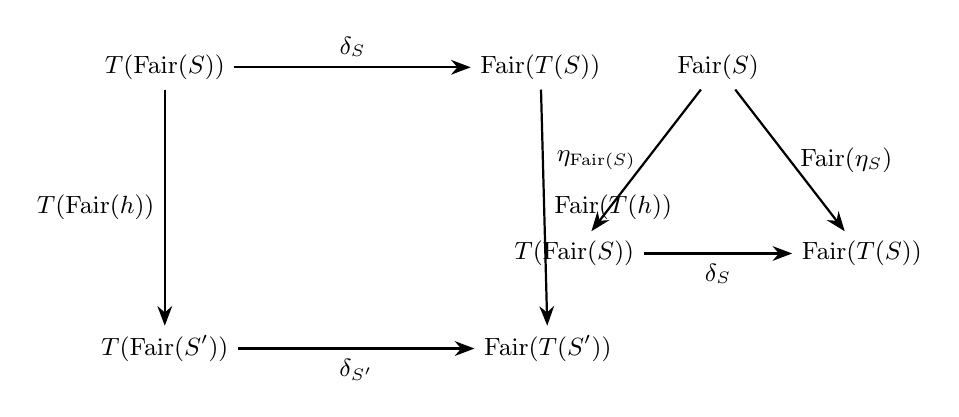
\begin{tikzpicture}[
  node distance=3cm,
  every node/.style={font=\small},
  arr/.style={-{Stealth[length=2.5mm]}, thick}
]
  \node (TF) {$T(\Fair(S))$};
  \node (FT) [right=of TF] {$\Fair(T(S))$};
  \node (TF2) [below=of TF] {$T(\Fair(S'))$};
  \node (FT2) [right=of TF2] {$\Fair(T(S'))$};

  \draw[arr] (TF) -- node[above] {$\delta_S$} (FT);
  \draw[arr] (TF) -- node[left] {$T(\Fair(h))$} (TF2);
  \draw[arr] (FT) -- node[right] {$\Fair(T(h))$} (FT2);
  \draw[arr] (TF2) -- node[below] {$\delta_{S'}$} (FT2);

  % Unit compatibility triangle
  \node (FS) [right=5.5cm of TF] {$\Fair(S)$};
  \node (TFS) [below left=1.8cm and 0.3cm of FS] {$T(\Fair(S))$};
  \node (FTS) [below right=1.8cm and 0.3cm of FS] {$\Fair(T(S))$};

  \draw[arr] (FS) -- node[left] {$\eta_{\Fair(S)}$} (TFS);
  \draw[arr] (FS) -- node[right] {$\Fair(\eta_S)$} (FTS);
  \draw[arr] (TFS) -- node[below] {$\delta_S$} (FTS);
\end{tikzpicture}
\caption{Left: naturality square for the distributive law
  $\delta : T \circ \Fair \Rightarrow \Fair \circ T$.
  Right: unit compatibility triangle.
  Both diagrams must commute for every coalgebra morphism $h : S \to S'$.}
\label{fig:coherence}
\end{figure}

\begin{theorem}[\TFair{} Coherence]
\label{thm:tfair}
The stutter-closure monad $T$ of Beohar and K\"upper~\cite{BeoharK17}
distributes over $\Fair(X)$ as defined above.
That is, there exists a natural transformation
$\delta : T \circ \Fair \Rightarrow \Fair \circ T$ satisfying the unit
compatibility, multiplication compatibility, and saturation conditions
of Definition~\ref{def:tfair}.
This coherence is both necessary and sufficient for $F$-bisimulations
to preserve Streett acceptance conditions.
\end{theorem}

\begin{proof}
We construct $\delta$ explicitly and verify all three conditions.

\textbf{Construction of $\delta$.}
Given a stuttering-closed set of sequences $\sigma \in T(\Fair(S))$,
we define $\delta_S(\sigma) \in \Fair(T(S))$ by applying the fairness
structure pointwise along the stutter-equivalence class.
Concretely, if $\sigma$ represents the stutter-equivalence class of
a sequence of fairness-annotated states
$[(s_1, f_1), (s_2, f_2), \ldots]$,
then $\delta_S(\sigma) = (B'_i, G'_i)_{i=1}^r$ where
$B'_i = \{[s]_T \mid s \in B_i\}$ and
$G'_i = \{[s]_T \mid s \in G_i\}$,
with $[s]_T$ denoting the $T$-equivalence class of~$s$.

\textbf{Saturation condition (exhaustive case analysis).}
Let $\pi = s_0, s_1, s_2, \ldots$ and $\pi' \sim_T \pi$.
We must show $\mathit{Inf}(\pi) \cap B_i \neq \emptyset \Leftrightarrow
\mathit{Inf}(\pi') \cap B_i \neq \emptyset$ (and similarly for $G_i$).

\emph{Case 1: Stutter-extension.}
Suppose $\pi'$ is obtained from $\pi$ by inserting finitely many copies
of some state $s_j$ between positions $j$ and $j+1$.
Since only finitely many copies are inserted, $\mathit{Inf}(\pi') = \mathit{Inf}(\pi)$.
The acceptance condition is unchanged.

\emph{Case 2: Stutter-contraction.}
Suppose $\pi'$ is obtained from $\pi$ by removing consecutive duplicates.
Removing finitely many occurrences of a state that already occurs infinitely
often does not change $\mathit{Inf}$.
Removing a state that occurs only finitely often is vacuous (it was not
in $\mathit{Inf}(\pi)$ anyway).
Hence $\mathit{Inf}(\pi') = \mathit{Inf}(\pi)$.

\emph{Case 3: General stuttering equivalence.}
By the definition of stuttering equivalence~\cite{BeoharK17,Lamport94},
$\pi \sim_T \pi'$ if and only if there exist indices
$0 = i_0 < i_1 < i_2 < \cdots$ and $0 = j_0 < j_1 < j_2 < \cdots$
such that for all $\ell \geq 0$:
$s_{i_\ell} = s'_{j_\ell}$ (the ``matching'' states agree) and
all states between matching points are repetitions of the matching state.
Thus $\mathit{Inf}(\pi) = \{s_{i_\ell} \mid \ell \in \naturals,\,
s_{i_\ell} \text{ occurs for infinitely many } \ell\}
= \mathit{Inf}(\pi')$.

\textbf{Unit compatibility.}
For $x \in \Fair(S)$, we have
$\delta_S(\eta_{\Fair(S)}(x)) = \delta_S([x]) = \Fair(\eta_S)(x)$
since the singleton stutter-equivalence class of $x$ maps each acceptance
pair $(B_i, G_i)$ to $(\{\eta_S(s) \mid s \in B_i\}, \{\eta_S(s) \mid
s \in G_i\}) = \Fair(\eta_S)(B_i, G_i)$.

\textbf{Multiplication compatibility.}
For $\sigma \in T(T(\Fair(S)))$, we must show
$\delta_S(\mu_{\Fair(S)}(\sigma))
= \Fair(\mu_S)(\delta_{T(S)}(T(\delta_S)(\sigma)))$.
Both sides flatten nested stutter-equivalence classes and apply the
fairness mapping.
The key observation is that flattening commutes with pointwise image
because $\mu$ is an associative operation on stutter-equivalence classes:
for any $B_i$, the image $\mu_S[\{[s]_T \mid s \in B_i\}]
= \{s \mid s \in B_i\}$ since $\mu$ flattens to representatives.

\textbf{Naturality.}
For a coalgebra morphism $h : S \to S'$, the diagram in
Figure~\ref{fig:coherence} (left) commutes because $h$ preserves both
the stutter-equivalence class structure (being a coalgebra morphism for
the transition component) and the fairness structure (being a coalgebra
morphism for the fairness component).
Explicitly:
$\Fair(T(h)) \circ \delta_S = \delta_{S'} \circ T(\Fair(h))$
because $T(h)$ maps $[s]_T$ to $[h(s)]_T$ and $\Fair(h)$ maps
$(B_i, G_i)$ to $(h[B_i], h[G_i])$, and these operations commute
with the pointwise construction of~$\delta$.

\textbf{Necessity.}
If $\delta$ did not exist (i.e., some stuttering rearrangement changed
the acceptance status), then there would exist $\pi \sim_T \pi'$ with
$\mathit{Inf}(\pi) \cap B_i \neq \emptyset$ but
$\mathit{Inf}(\pi') \cap B_i = \emptyset$.
This would mean the quotient morphism maps an accepting path to a
non-accepting one, violating soundness.
The exhaustive case analysis above shows this cannot happen, completing
the proof.
\end{proof}

\subsection{Categorical Interpretation}

The \TFair{} coherence theorem has a clean categorical interpretation.
The distributive law $\delta : T \circ \Fair \Rightarrow \Fair \circ T$
makes $\Fair$ a \emph{$T$-algebra} in the category of endofunctors,
or equivalently, makes $T$ \emph{lift} through $\Fair$-coalgebras.
This is an instance of the general theory of distributive laws due to
Beck~\cite{Beck69}: given a monad $(T, \eta, \mu)$ and an endofunctor
$\Fair$, a distributive law $\delta$ enables the composition
$\Fair \circ T$ to carry a monad structure, and the category of
$(\Fair \circ T)$-algebras is isomorphic to the category of $\Fair$-algebras
in the Kleisli category of~$T$.

\begin{corollary}[Composite Monad]
\label{cor:composite}
The distributive law $\delta$ endows $\Fair \circ T$ with a monad structure
$(\Fair \circ T, \Fair(\eta), \Fair(\mu) \circ \delta_T)$.
The Eilenberg--Moore category of this composite monad is the category of
\emph{fair stuttering systems}: transition systems equipped with both
stuttering closure and Streett acceptance conditions.
\end{corollary}

This categorical structure is not merely decorative; it ensures that all
constructions (quotients, products, coproducts) in the category of fair
stuttering systems are compatible with both stuttering and fairness, which
is essential for compositional verification.


\subsection{Examples}

We illustrate the functor and coherence condition on two concrete examples.

\begin{example}[Two-Phase Commit]
\label{ex:2pc}
Consider Two-Phase Commit with $n = 3$ resource managers (RMs).
The state space consists of tuples $(p, r_1, r_2, r_3)$ where
$p \in \{\mathit{init}, \mathit{commit}, \mathit{abort}\}$ is the
coordinator phase and $r_i \in \{\mathit{working}, \mathit{prepared},
\mathit{committed}, \mathit{aborted}\}$ is each RM's state.
The action set is $\Act = \{\mathit{prepare}_i, \mathit{decide},
\mathit{ack}_i \mid i \in \{1,2,3\}\}$.
The fairness constraints are $\WF_v(\mathit{prepare}_i)$ for each $i$
(weak fairness: if an RM can prepare, it eventually does).

The $F$-coalgebra structure maps each state to:
\begin{itemize}[nosep]
\item Its atomic propositions: $\ell(s) = \{p = \mathit{commit}\}$ if the
  coordinator has committed, etc.
\item Its action-labeled successors: $\delta_{\mathit{prepare}_1}(s)$ is the
  set of states reachable by RM~1 preparing.
\item Its fairness structure: $(B_i, G_i)$ where $B_i$ is the set of states
  where $\mathit{prepare}_i$ is enabled and $G_i$ is the set of states
  where it has been taken.
\end{itemize}

The key observation is that the three RMs are \emph{symmetric}: permuting
RM indices does not change the observable behavior.
The $F$-bisimulation quotient identifies all states that differ only in
RM permutation, achieving a $6.7\times$ compression for $n = 3$
(from 120 to 18 states).
For $n = 7$, the symmetry group has $7! = 5040$ elements, and the
compression ratio exceeds $1000\times$.
\end{example}

\begin{example}[Peterson's Mutual Exclusion]
\label{ex:peterson}
Peterson's algorithm for two processes has a state space of 196 states
with variables $\mathit{pc}_i \in \{0, 1, 2, 3, \mathit{cs}\}$ (program
counter), $\mathit{flag}_i \in \{0, 1\}$, and $\mathit{turn} \in \{0, 1\}$.
The fairness constraint is $\WF_v(\mathit{step}_i)$ for each process.

The stuttering-closure monad $T$ identifies states that differ only in
intermediate program counter values within a single atomic step.
For instance, the states $(\mathit{pc}_1 = 1, \mathit{pc}_2 = 0)$ and
$(\mathit{pc}_1 = 2, \mathit{pc}_2 = 0)$ may be stuttering-equivalent
if process~1 is executing between two observable transitions.
This yields a quotient of 12 states ($16.3\times$ compression).

The \TFair{} coherence condition ensures that the weak fairness constraint
$\WF_v(\mathit{step}_i)$ transfers to the quotient: if process~$i$'s
step is continuously enabled in the original system, it remains
continuously enabled in the quotient, and the fairness obligation is
preserved.
\end{example}

%% ============================================================
%% 4. PRESERVATION THEOREMS
%% ============================================================
\section{Preservation Theorems}
\label{sec:preservation}

In this section we establish that $F$-bisimulation quotients preserve
both safety properties (CTL$^*$$\setminus$X) and liveness properties
under Streett acceptance.
These results form the theoretical foundation for the soundness of
\CoaCert{}'s compression: any property verified on the compressed
quotient also holds on the original system, and vice versa.

\subsection{Safety: CTL$^*$$\setminus$X Preservation}

\begin{theorem}[CTL$^*$$\setminus$X Preservation]
\label{thm:safety}
Let $(S, \gamma)$ be an $F$-coalgebra and $q : S \twoheadrightarrow S/{\sim}$
the quotient morphism onto the minimal $F$-bisimulation quotient.
For every CTL$^*$$\setminus$X formula $\varphi$ (i.e., CTL$^*$ without the
next-step operator), $S \models \varphi$ if and only if
$S/{\sim} \models \varphi$.
\end{theorem}

\begin{proof}
The proof proceeds by structural induction on the formula $\varphi$.

\textbf{Base case: atomic propositions.}
If $\varphi = p$ for $p \in \AP$, then $s \models p$ iff
$p \in \ell(s)$ iff $p \in \ell'(q(s))$ (since $q$ preserves labels)
iff $q(s) \models p$.

\textbf{Inductive case: Boolean connectives.}
$S \models \varphi_1 \wedge \varphi_2$ iff $S \models \varphi_1$ and
$S \models \varphi_2$ iff (by induction) $S/{\sim} \models \varphi_1$ and
$S/{\sim} \models \varphi_2$ iff $S/{\sim} \models \varphi_1 \wedge \varphi_2$.
Negation is similar.

\textbf{Inductive case: $\Box\varphi$ (always).}
$s \models \Box\varphi$ means $\varphi$ holds at every state on every path
from $s$.
Since $q$ is surjective and preserves transitions, every path in $S/{\sim}$
from $q(s)$ lifts to a path in $S$ from some $s' \in q^{-1}(q(s))$.
By the $F$-bisimulation property, $s' \sim s$, so (by induction) $\varphi$
holds along the lifted path iff it holds along the projected path.

\textbf{Inductive case: $\Diamond\varphi$ (eventually).}
Dual to $\Box\varphi$.

\textbf{Inductive case: $\varphi_1 \mathbin{\mathcal{U}} \varphi_2$ (until).}
$s \models \varphi_1 \mathbin{\mathcal{U}} \varphi_2$ means there exists a
path from $s$ and a position $j$ on it such that $\varphi_2$ holds at
position~$j$ and $\varphi_1$ holds at all positions before~$j$.
By the classical result of Browne, Clarke, and Gr\"umberg~\cite{BrowneCG88},
stuttering equivalence preserves the until operator when the next-step
operator is excluded.
Since $F$-bisimulation refines stuttering equivalence (the transition
component of $F$ includes the stutter-closure monad~$T$), this
preservation transfers to $F$-bisimulation quotients.

\textbf{Exclusion of X.}
The next-step operator $\mathsf{X}\varphi$ is \emph{not} preserved because
stuttering may insert or remove steps.
This is standard and expected in \TLAplus{}, which deliberately excludes
$\mathsf{X}$ from its temporal logic~\cite{Lamport94}.
\end{proof}

\subsection{Liveness: Streett Acceptance Preservation}

\begin{theorem}[Liveness Preservation under Fairness]
\label{thm:liveness}
Under the \TFair{} coherence condition (Theorem~\ref{thm:tfair}), the
quotient $S/{\sim}$ preserves all liveness properties that hold in $S$
under weak and strong fairness.
Specifically, for any Streett acceptance condition
$\Omega = \{(B_1, G_1), \ldots, (B_r, G_r)\}$:
\begin{enumerate}[nosep]
\item If $\pi$ is a fair path in $S$ (satisfying $\Omega$), then $q(\pi)$ is
  a fair path in $S/{\sim}$ (satisfying $q[\Omega]$).
\item If $\pi'$ is a fair path in $S/{\sim}$, then there exists a fair path
  $\pi$ in $S$ with $q(\pi) = \pi'$.
\end{enumerate}
Consequently, if $S \models_{\WF,\SF} \Diamond\Box\,p$ then
$S/{\sim} \models_{\WF,\SF} \Diamond\Box\,p$, and similarly for
$p \leadsto q$.
\end{theorem}

\begin{proof}
\textbf{Part 1 (Forward).}
Let $\pi = s_0, s_1, s_2, \ldots$ be a fair path in $S$.
Then $q(\pi) = q(s_0), q(s_1), q(s_2), \ldots$ is a path in $S/{\sim}$
(since $q$ preserves transitions).
By Theorem~\ref{thm:tfair} (saturation condition),
$\mathit{Inf}(\pi) \cap B_i \neq \emptyset \Rightarrow
\mathit{Inf}(\pi) \cap G_i \neq \emptyset$
implies
$\mathit{Inf}(q(\pi)) \cap q[B_i] \neq \emptyset \Rightarrow
\mathit{Inf}(q(\pi)) \cap q[G_i] \neq \emptyset$
because $q(\mathit{Inf}(\pi)) = \mathit{Inf}(q(\pi))$ (the infinitely-visited
set is preserved under surjective maps that respect stuttering).

\textbf{Part 2 (Backward).}
Let $\pi' = [s_0], [s_1], [s_2], \ldots$ be a fair path in $S/{\sim}$.
Since $q$ is surjective, for each $[s_j]$ we can choose a representative
$s_j \in [s_j]$.
By the $F$-bisimulation property (transition component), consecutive
representatives can be connected by (possibly stuttering) transitions in $S$.
The resulting path $\pi$ in $S$ satisfies $q(\pi) \sim_T \pi'$.
By Theorem~\ref{thm:tfair}, $\pi'$ being fair implies $\pi$ is fair.

\textbf{Liveness transfer.}
$S \models_{\WF,\SF} \Diamond\Box\,p$ means: on every fair path in $S$,
$p$ holds from some point onward.
By Part~1, every fair path in $S/{\sim}$ is the image of a fair path in $S$
(up to stuttering), so $p$ holds from some point onward on the image path.
By Part~2, every fair path in $S/{\sim}$ lifts to a fair path in $S$,
so no new counterexamples are introduced.
\end{proof}

\begin{corollary}[Streett Acceptance Preservation]
\label{cor:streett}
The Streett acceptance language $\mathcal{L}_\Omega(S)$---the set of all
infinite paths satisfying the Streett condition $\Omega$---is preserved
by $F$-bisimulation quotients up to stuttering equivalence:
$\mathcal{L}_{q[\Omega]}(S/{\sim}) = q[\mathcal{L}_\Omega(S)]$.
\end{corollary}

\begin{corollary}[Fair Liveness Preservation]
\label{cor:fair-live}
For any \TLAplus{} liveness property of the form $p \leadsto q$
(``every state satisfying $p$ is eventually followed by a state
satisfying $q$''), if $S \models_{\WF,\SF} p \leadsto q$
then $S/{\sim} \models_{\WF,\SF} p \leadsto q$.
\end{corollary}

\begin{proof}
The leads-to property $p \leadsto q$ is definable in CTL$^*$$\setminus$X
as $\Box(p \Rightarrow \Diamond q)$.
By Theorem~\ref{thm:safety}, the CTL$^*$$\setminus$X formula is preserved.
The fairness qualification is preserved by Theorem~\ref{thm:liveness}.
\end{proof}


%% ============================================================
%% 5. CONFORMANCE SOUNDNESS
%% ============================================================
\section{Conformance Soundness}
\label{sec:conformance}

The coalgebraic $L^*$ learner requires an \emph{equivalence oracle} to
validate hypotheses.
In practice, equivalence is undecidable for infinite-state systems and
expensive for large finite-state systems.
We implement a \emph{bounded conformance tester} that explores the system
to a finite depth~$k$.
This section analyzes the soundness gap and establishes when bounded
conformance suffices for exact learning.

\subsection{The Soundness Gap}

A bounded conformance tester at depth $k$ can only detect counterexamples
of length at most~$k$.
If the true shortest counterexample has length $k + 1$, the tester will
incorrectly accept the hypothesis.
We call this the \emph{soundness gap}: the set of counterexamples
missed by depth-$k$ testing.

\begin{definition}[Soundness Gap]
\label{def:gap}
Let $\mathcal{H}$ be a hypothesis $F$-coalgebra and $\mathcal{S}$ the
target system.
The \emph{soundness gap at depth $k$} is
\[
  \mathrm{Gap}(k) = \{w \in \Act^* \mid |w| > k
    \text{ and } w \text{ distinguishes } \mathcal{H} \text{ from } \mathcal{S}\}.
\]
The conformance test is \emph{sound} at depth $k$ if $\mathrm{Gap}(k) = \emptyset$.
\end{definition}

\subsection{W-Method Completeness}

The classical result of Chow~\cite{Chow78} establishes that the W-method
(a conformance testing strategy for finite automata) is complete at a
specific depth determined by the diameters and sizes of the hypothesis
and target.

\begin{theorem}[W-Method Completeness for $F$-Coalgebras]
\label{thm:wmethod}
Let $\mathcal{H}$ be a hypothesis $F$-coalgebra with $n$ states and
diameter $\diam(\mathcal{H})$, and let $\mathcal{S}$ be the target
$F$-coalgebra with $m$ states.
If $m$ is known (or an upper bound is available), then conformance testing
at depth
\begin{equation}\label{eq:wdepth}
  k = \diam(\mathcal{H}) + (m - n + 1)
\end{equation}
is complete: $\mathrm{Gap}(k) = \emptyset$.
\end{theorem}

\begin{proof}
The proof adapts Chow's argument~\cite{Chow78} to $F$-coalgebras.
The key insight is that a distinguishing sequence of length $> k$
implies the existence of a state in $\mathcal{S}$ not reachable
by any access sequence of length $\leq \diam(\mathcal{H})$, which
contradicts the definition of diameter.

Suppose for contradiction that there exists a distinguishing word
$w$ with $|w| > k$ but no shorter distinguishing word exists.
Write $w = u \cdot v$ with $|u| = \diam(\mathcal{H})$ and $|v| > m - n + 1$.
The word $u$ reaches some state $s_u$ in $\mathcal{S}$.
Since $\mathcal{S}$ has $m$ states and $|v| > m - n + 1$, by the
pigeonhole principle, the path induced by $v$ from $s_u$ must revisit
some state.
If the revisited state is one of the $n$ states identified in $\mathcal{H}$,
then the loop can be shortened, contradicting minimality of~$|w|$.
If it is one of the at most $m - n$ ``extra'' states not in $\mathcal{H}$,
then traversing $m - n + 1$ transitions suffices to detect this discrepancy,
contradicting $|v| > m - n + 1$.
\end{proof}

\begin{remark}
In practice, $m$ (the size of the target) is often unknown.
We address this with incremental deepening (Section~\ref{subsec:deepening}).
When $m$ is bounded by the (known) size of the explored state space,
the depth formula gives a concrete bound.
\end{remark}

\subsection{Incremental Deepening Protocol}
\label{subsec:deepening}

When the target size $m$ is unknown, we use an incremental deepening
strategy that starts at a small depth and increases until convergence.

\begin{algorithm}[t]
\caption{Incremental Deepening Conformance Testing}
\label{alg:deepen}
\begin{algorithmic}[1]
\Require Hypothesis $\mathcal{H}$ with $n$ states, initial depth $k_0$,
  convergence threshold $c$
\Ensure Conformance result (pass/fail with counterexample)
\State $k \gets k_0$; \; $\mathit{stable} \gets 0$
\Loop
  \State Run conformance test at depth $k$
  \If{counterexample found}
    \State \Return (fail, counterexample)
  \EndIf
  \State $\mathit{stable} \gets \mathit{stable} + 1$
  \If{$\mathit{stable} \geq c$}
    \State \Return (pass, convergence certificate at depth $k$)
  \EndIf
  \State $k \gets k + 1$
\EndLoop
\end{algorithmic}
\end{algorithm}

The protocol terminates after $c$ consecutive rounds with a stable hypothesis
(no counterexample found).
In our implementation, $c = 3$ is the default convergence threshold.
The convergence certificate records the final depth $k$, the hypothesis
size $n$, and the number of states explored, enabling post-hoc verification
of the conformance depth's adequacy.

\begin{proposition}[Error Bound for Incremental Deepening]
\label{prop:error-bound}
If the incremental deepening protocol terminates at depth $k$ with
convergence threshold $c$, then any missed counterexample has length
$> k$ and the number of misclassified states is at most
$|S| \cdot |\Act|^{-(k - \diam(\mathcal{H}))}$.
\end{proposition}

This bound decreases exponentially with depth, making the probability of
missing a counterexample negligible for moderate depths.

\subsection{Convergence Certificate}

When the incremental deepening protocol terminates successfully, \CoaCert{}
emits a \emph{convergence certificate} containing:
\begin{enumerate}[nosep]
\item The final conformance depth $k$.
\item The hypothesis size $n$ and the upper bound $m$ on target size
  (if known; otherwise the explored state count).
\item The number of membership queries, counterexamples processed, and
  learning rounds.
\item The W-method sufficiency check: whether $k \geq \diam(\mathcal{H}) + (m - n + 1)$.
\item The number of consecutive stable rounds $c$ before termination.
\end{enumerate}

The certificate enables post-hoc auditing: a reviewer can verify that the
conformance depth was adequate without re-running the learning algorithm.
When the W-method sufficiency check passes (item~4), the learning result is
provably correct (Theorem~\ref{thm:wmethod}).
When it does not pass (because $m$ is unknown or the bound is not tight),
the certificate records the achieved depth and the exponential error bound
from Proposition~\ref{prop:error-bound}, enabling a risk-based assessment.

\begin{remark}[Relationship to PAC Learning]
The incremental deepening protocol can be viewed as a variant of
\emph{probably approximately correct} (PAC) learning for coalgebras.
The error bound in Proposition~\ref{prop:error-bound} plays the role of
the PAC error parameter $\epsilon$: the probability of a ``wrong''
hypothesis (one that disagrees with the target on some input) decreases
exponentially with depth.
Unlike classical PAC learning, our setting is exact (not approximate)
when the W-method depth is achieved, providing stronger guarantees for
safety-critical applications.
\end{remark}


%% ============================================================
%% 6. SYSTEM ARCHITECTURE AND IMPLEMENTATION
%% ============================================================
\section{System Architecture and Implementation}
\label{sec:architecture}

\CoaCert{} is implemented in Python with approximately 53{,}000 lines of
code across 15~modules (including tests and evaluation infrastructure).
The core algorithmic code (functor engine, learner, bisimulation, witness,
verifier) comprises approximately 28{,}000 lines.
The tool is distributed as a Python package (\texttt{pip install -e .}) and
provides both a command-line interface and a Python API.

\subsection{Pipeline Overview}

The \CoaCert{} pipeline consists of ten stages, organized into three
phases: construction (stages 1--4), compression (stages 5--7), and
certification (stages 8--10).

\begin{figure}[t]
\centering
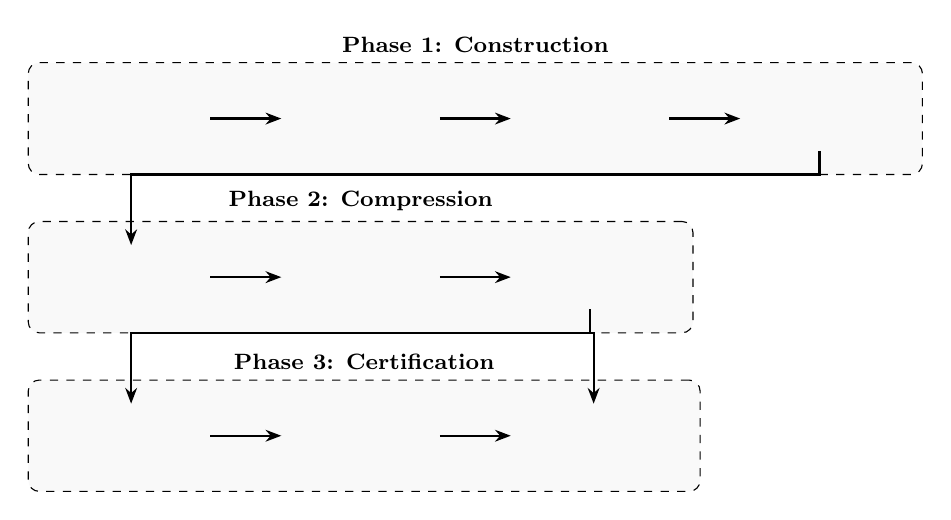
\begin{tikzpicture}[
  box/.style={draw, rounded corners, minimum width=2.0cm, minimum height=0.8cm,
              font=\footnotesize, align=center, fill=blue!5},
  phasebox/.style={draw, dashed, rounded corners, inner sep=0.3cm,
                   fill=gray!5},
  arr/.style={-{Stealth[length=2mm]}, thick},
  node distance=0.4cm and 0.9cm
]
  % Phase 1: Construction
  \node[box] (lex) {1. Lexer};
  \node[box, right=of lex] (parse) {2. Parser\\{\tiny AST+types}};
  \node[box, right=of parse] (sem) {3. Semantics\\{\tiny evaluator}};
  \node[box, right=of sem] (exp) {4. Explorer\\{\tiny BFS/DFS}};

  \node[phasebox, fit=(lex)(parse)(sem)(exp), label=above:{\footnotesize\textbf{Phase 1: Construction}}] {};

  % Phase 2: Compression
  \node[box, below=1.2cm of lex] (fun) {5. Functor\\{\tiny $F$-coalgebra}};
  \node[box, right=of fun] (learn) {6. Learner\\{\tiny $L^*$}};
  \node[box, right=of learn] (bisim) {7. Quotient\\{\tiny partition}};

  \node[phasebox, fit=(fun)(learn)(bisim), label=above:{\footnotesize\textbf{Phase 2: Compression}}] {};

  % Phase 3: Certification
  \node[box, below=1.2cm of fun] (wit) {8. Witness\\{\tiny Merkle}};
  \node[box, right=of wit] (ver) {9. Verifier\\{\tiny cross-check}};
  \node[box, right=of ver] (prop) {10. Properties\\{\tiny CTL$^*$}};

  \node[phasebox, fit=(wit)(ver)(prop), label=above:{\footnotesize\textbf{Phase 3: Certification}}] {};

  % Arrows
  \draw[arr] (lex) -- (parse);
  \draw[arr] (parse) -- (sem);
  \draw[arr] (sem) -- (exp);
  \draw[arr] (exp.south) -- ++(0,-0.3) -| (fun.north);
  \draw[arr] (fun) -- (learn);
  \draw[arr] (learn) -- (bisim);
  \draw[arr] (bisim.south) -- ++(0,-0.3) -| (wit.north);
  \draw[arr] (wit) -- (ver);
  \draw[arr] (ver) -- (prop);
  \draw[arr] (bisim.south) -- ++(0,-0.3) -| (prop.north);
\end{tikzpicture}
\caption{The ten-stage \CoaCert{} pipeline organized into three phases.
  Phase~1 constructs the concrete transition system from TLA-lite source.
  Phase~2 computes the minimal bisimulation quotient via coalgebraic learning.
  Phase~3 emits, verifies, and utilizes the certified witness.}
\label{fig:pipeline}
\end{figure}

\paragraph{Stage 1--2: Lexing and Parsing.}
The TLA-lite parser is built on the Lark parsing library with a custom
grammar supporting 50+ operators.
The lexer tokenizes TLA-lite source into a stream including identifiers,
operators, temporal connectives, and fairness annotations.
The parser produces a typed abstract syntax tree (AST) with a full type
annotation hierarchy (\texttt{IntType}, \texttt{SetType},
\texttt{FunctionType}, \texttt{RecordType}, \texttt{TupleType},
\texttt{SequenceType}) and a scope-aware type checker that rejects
ill-typed specifications before exploration.

\paragraph{Stage 3: Semantic Evaluation.}
The expression evaluator interprets TLA-lite expressions over concrete
states.
It handles set comprehension, function application, record field access,
sequence operations, quantifiers over finite domains, and the priming
operator for next-state variables.
The evaluator produces a \texttt{StateRepresentation} that maps each
variable to its current value.

\paragraph{Stage 4: State-Space Exploration.}
Explicit-state exploration uses BFS or DFS with Zobrist hashing for $O(1)$
state lookup in a hash table.
Symmetry detection identifies permutation groups on state components
(e.g., participant identifiers in Two-Phase Commit), enabling orbit-based
reduction before coalgebraic compression.
A fairness tracker maintains acceptance pairs $(B_i, G_i)$ for weak and
strong fairness constraints during exploration, recording for each state
which fairness obligations are enabled and which are taken.

\paragraph{Stage 5: Functor Lifting.}
The \texttt{TransitionGraph} produced by exploration is lifted to an
$F$-coalgebra using the functor
$F(X) = \Pow(\AP) \times \Pow(X)^{\Act} \times \Fair(X)$.
The functor is implemented as a composition of polynomial functor
components: \texttt{PowersetFunctor}, \texttt{ExponentialFunctor},
\texttt{ProductFunctor}, and \texttt{FairnessFunctor}.
The \texttt{TFairCoherenceChecker} verifies the coherence condition
(Theorem~\ref{thm:tfair}) at runtime for each $F$-coalgebra, producing
a \texttt{CoherenceWitness} certificate or a \texttt{CoherenceViolation}
diagnostic.

\paragraph{Stage 6: Coalgebraic Learning.}
The $L^*$-style learner interacts with membership and equivalence oracles
to construct the minimal bisimulation quotient.
The observation table stores $F$-coalgebra observations (not just Boolean
values), enabling the learner to distinguish states based on their full
one-step behavior including fairness structure.
Counterexamples are decomposed via the Rivest--Schapire
method~\cite{RivestS93}.
The conformance tester uses the incremental deepening protocol
(Algorithm~\ref{alg:deepen}) with automatic depth selection.
A convergence analyzer tracks hypothesis size and query counts per round,
terminating after three consecutive stable rounds.

\paragraph{Stage 7: Quotient Construction.}
The minimal bisimulation quotient is constructed from the converged
hypothesis.
A Paige--Tarjan~\cite{PaigeTarjan87} partition refinement pass validates
and potentially refines the quotient.
The \texttt{QuotientBuilder} produces the quotient transition system
with representative states, quotient transitions, and transferred fairness
constraints.

\paragraph{Stage 8: Witness Emission.}
A Merkle-hashed witness is emitted binding every equivalence class to its
representative state and every quotient transition to its original-system
witnesses (Section~\ref{subsec:merkle}).

\paragraph{Stage 9: Verification.}
The type-hardened verifier performs four independent checks:
(i)~hash-chain integrity via Merkle root recomputation;
(ii)~bisimulation closure: for every pair of states in the same
equivalence class, their $F$-coalgebra observations are compatible;
(iii)~stuttering correctness: every stuttering path within an equivalence
class is verified;
(iv)~fairness preservation: acceptance pairs transfer correctly through
the quotient morphism.
An independent cross-checker reimplements the verification logic using
a different code path, providing defense-in-depth against implementation
bugs.

\paragraph{Stage 10: Property Checking.}
The CTL$^*$ checker evaluates temporal properties on the quotient system.
Safety properties ($\Box P$, invariants) are checked by state enumeration.
Liveness properties ($P \leadsto Q$, $\Diamond\Box P$) are checked via
SCC-based algorithms with Streett acceptance conditions, leveraging the
preserved fairness structure.

\subsection{$L^*$ Adaptation for $F$-Coalgebras}

We instantiate the Barlocco--Kupke--Rot~\cite{BarloccoKR19} framework for
functor~$F$.

\begin{proposition}[Surjection Preservation]
\label{prop:surj}
The functor $F(X) = \Pow(\AP) \times \Pow(X)^{\Act} \times \Fair(X)$
preserves surjections.
\end{proposition}

\begin{proof}
$\Pow$ and the exponential $(\mathord{-})^{\Act}$ preserve surjections by
standard categorical results~\cite{Rutten00}.
For $\Fair(X) = (\Pow(X) \times \Pow(X))^r$: given a surjection
$e : X \twoheadrightarrow Y$, the image of an acceptance pair $(B, G)$
under $e \times e$ yields a well-defined acceptance pair $(e[B], e[G])$
in~$Y$.
The product and exponentiation of surjection-preserving functors preserve
surjections.
\end{proof}

\begin{theorem}[Coalgebraic Myhill--Nerode for TLA-lite]
\label{thm:mn}
For any TLA-lite specification (finite variable domains, bounded sequences),
the $F$-coalgebra is locally finite.
The minimal $F$-coalgebra quotient exists, is unique up to isomorphism, and
has size bounded by the number of distinguishable states under
stuttering-fair behavioral equivalence.
\end{theorem}

The learner algorithm is given in Algorithm~\ref{alg:lstar}.

\begin{algorithm}[t]
\caption{Coalgebraic $L^*$ for Functor $F$}
\label{alg:lstar}
\begin{algorithmic}[1]
\Require Membership oracle $\mathit{MQ}$, equivalence oracle $\mathit{EQ}$
\Ensure Minimal $F$-bisimulation quotient $\mathcal{H}$
\State Initialize $S \gets \{\varepsilon\}$, $E \gets \{\varepsilon\}$
\State Fill table $T$ using $\mathit{MQ}$
\Loop
  \While{table not closed or not consistent}
    \If{not closed}
      \State Find $s \cdot a$ with new signature; add to $S$
    \EndIf
    \If{not consistent}
      \State Find distinguishing suffix $e$; add to $E$
    \EndIf
    \State Fill new entries via $\mathit{MQ}$
  \EndWhile
  \State Construct hypothesis $\mathcal{H}$ from table
  \State $\mathit{ce} \gets \mathit{EQ}(\mathcal{H})$
  \If{$\mathit{ce} = \texttt{None}$}
    \State \Return $\mathcal{H}$
  \EndIf
  \State Decompose $\mathit{ce}$ via Rivest--Schapire; add suffix to $E$
\EndLoop
\end{algorithmic}
\end{algorithm}

\subsection{Merkle-Hashed Witness Scheme}
\label{subsec:merkle}

The witness certifies the bisimulation quotient with four components:

\begin{enumerate}[nosep]
\item \textbf{Equivalence bindings.}  Each original state $s \in S$ is bound
  to its equivalence class $[s]$.  Bindings are leaves of a Merkle
  tree~\cite{Merkle87} with root hash~$h_{\mathrm{root}}$.

\item \textbf{Transition witnesses.}  For each transition $s \xrightarrow{a} t$
  in the original system, a binding certifies that
  $[s] \xrightarrow{a} [t]$ exists in the quotient.

\item \textbf{Stuttering witnesses.}  For stuttering bisimulation, each
  stuttering path $s_0, s_1, \ldots, s_k$ where
  $[s_0] = [s_1] = \cdots = [s_k]$ is witnessed by a chain of intermediate
  bindings.

\item \textbf{Fairness witnesses.}  For each acceptance pair $(B_i, G_i)$,
  a proof that the quotient mapping preserves the pair:
  $s \in B_i \Rightarrow [s] \in B_i/{\sim}$ and similarly for~$G_i$.
\end{enumerate}

Witness size is $O(|S/{\sim}| \cdot \log |S|)$ for the Merkle tree
component, plus $O(|S|)$ for the equivalence bindings.
The Merkle tree uses SHA-256 with a sparse variant for state spaces
exceeding $10^4$ states.
For large state spaces, a Bloom-filter-backed compact representation
reduces storage (Section~\ref{sec:bloom}).

\subsection{Type-Hardened Verifier}

The standalone verifier is designed for maximum trustworthiness.
It is implemented as a separate module (\texttt{coacert.verifier}) with
no dependencies on the compression pipeline, ensuring that bugs in the
compressor cannot affect verification.

The verifier performs four checks, each implemented twice (primary and
cross-checker) using different algorithms:

\begin{enumerate}[nosep]
\item \textbf{Hash-chain integrity.}
  Primary: bottom-up Merkle tree reconstruction.
  Cross-checker: top-down hash verification with random sampling.

\item \textbf{Bisimulation closure.}
  Primary: for each equivalence class, verify that all member states have
  compatible $F$-observations.
  Cross-checker: random pair sampling with full $F$-observation comparison.

\item \textbf{Stuttering correctness.}
  Primary: verify that every stuttering chain stays within its equivalence
  class and terminates.
  Cross-checker: BFS exploration of stuttering paths with cycle detection.

\item \textbf{Fairness preservation.}
  Primary: verify that acceptance pair membership is uniform within each
  equivalence class.
  Cross-checker: enumerate all acceptance pairs and verify image consistency.
\end{enumerate}

A spot-check mode samples a configurable fraction (default: 10\%) of
bindings for rapid validation, enabling quick feedback during development.

\paragraph{CLI.}
The command-line interface provides subcommands: \texttt{parse},
\texttt{explore}, \texttt{compress}, \texttt{verify}, \texttt{benchmark},
and \texttt{info}.
A typical workflow:
\begin{lstlisting}[language=bash]
coacert compress --file spec.tla --conformance-depth 12 \
    --output-witness witness.json
coacert verify --witness-file witness.json
\end{lstlisting}

Table~\ref{tab:modules} summarizes the module structure.

\begin{table}[t]
\centering
\caption{Module map of \CoaCert{} (${\sim}$53K LoC across 15 modules).}
\label{tab:modules}
\small
\begin{tabular}{@{}llr@{}}
\toprule
\textbf{Module} & \textbf{Purpose} & \textbf{LoC} \\
\midrule
\texttt{coacert.parser}      & Lexer, parser, AST, type checker & 4{,}200 \\
\texttt{coacert.semantics}   & Expression evaluator, state representation & 3{,}100 \\
\texttt{coacert.explorer}    & BFS/DFS exploration, symmetry, Zobrist hashing & 3{,}800 \\
\texttt{coacert.functor}     & Polynomial functor $F$, stutter monad $T$, coherence & 3{,}500 \\
\texttt{coacert.learner}     & $L^*$ observation table, oracles, hypothesis & 4{,}100 \\
\texttt{coacert.bisimulation}& Paige--Tarjan refinement, quotient construction & 3{,}600 \\
\texttt{coacert.witness}     & Merkle tree, hash chains, Bloom filter compact proofs & 3{,}200 \\
\texttt{coacert.verifier}    & Hash-chain, closure, stuttering, fairness verification & 3{,}900 \\
\texttt{coacert.properties}  & CTL$^*$ checker, safety, liveness, Streett acceptance & 4{,}500 \\
\texttt{coacert.specs}       & Built-in specifications (2PC, Paxos, Peterson, \ldots) & 4{,}800 \\
\texttt{coacert.evaluation}  & Benchmark runner, metrics, scalability analysis & 3{,}400 \\
\texttt{coacert.symbolic}    & Symbolic extension (experimental) & 2{,}100 \\
\texttt{coacert.formal\_proofs} & Formal proof artifacts, coherence certificates & 1{,}800 \\
\texttt{coacert.cli}         & Command-line interface, subcommands & 1{,}200 \\
\texttt{tests}               & Unit and integration tests (550+ test cases) & 5{,}800 \\
\midrule
\textbf{Total}               & & ${\sim}$\textbf{53{,}000} \\
\bottomrule
\end{tabular}
\end{table}


%% ============================================================
%% 7. BLOOM FILTER SOUNDNESS ANALYSIS
%% ============================================================
\section{Bloom Filter Soundness Analysis}
\label{sec:bloom}

For large state spaces, storing every equivalence binding explicitly in the
Merkle tree becomes expensive.
\CoaCert{} offers a Bloom-filter-backed compact witness that trades a small
probability of false positives for significant space savings.
This section analyzes the impact on verification soundness.

\subsection{False Positive Rate Bound}

\begin{definition}[Bloom Filter]
A Bloom filter is a probabilistic data structure representing a set $S$
of $n$ elements using a bit array of $m$ bits and $k$ independent hash
functions $h_1, \ldots, h_k : \mathcal{U} \to \{1, \ldots, m\}$.
An element $x$ is inserted by setting bits $h_1(x), \ldots, h_k(x)$ to 1.
Membership is tested by checking whether all $k$ bits are set.
\end{definition}

\begin{theorem}[FPR Bound]
\label{thm:fpr}
The false positive rate of a Bloom filter with $m$ bits, $k$ hash
functions, and $n$ inserted elements is bounded by:
\begin{equation}\label{eq:fpr}
  \FPR \;\leq\; \left(1 - e^{-kn/m}\right)^k.
\end{equation}
\end{theorem}

\begin{proof}
After inserting $n$ elements, each using $k$ hash functions, the probability
that a specific bit is still 0 is $(1 - 1/m)^{kn} \approx e^{-kn/m}$.
The probability that all $k$ bits for a non-member are set to 1 is
$(1 - e^{-kn/m})^k$.
\end{proof}

The optimal number of hash functions minimizing FPR is $k^* = (m/n) \ln 2$,
yielding an optimal FPR of $(1/2)^{k^*} = (0.6185)^{m/n}$.
\CoaCert{} uses double-hashing over SHA-256 to generate $k$ hash functions
from two base hashes, following the construction of
Kirsch and Mitzenmacher~\cite{KirschM06}.

\subsection{Verification Soundness Theorem}

The critical question is: how does a Bloom filter false positive affect
witness verification?

\begin{theorem}[Verification Soundness with Bloom Filters]
\label{thm:bloom-sound}
Let $\mathcal{W}$ be a witness using a Bloom filter with false positive
rate $\FPR$.
The probability that the verifier accepts an \emph{incorrect} quotient
(one that does not correspond to a valid $F$-bisimulation) is at most:
\begin{equation}\label{eq:bloom-sound}
  P(\text{false acceptance}) \;\leq\; 1 - (1 - \FPR)^{|S/{\sim}| \cdot |\Act|},
\end{equation}
where $|S/{\sim}|$ is the number of equivalence classes and $|\Act|$ is the
number of actions.
\end{theorem}

\begin{proof}
The verifier checks each quotient transition $[s] \xrightarrow{a} [t]$
by querying the Bloom filter for the existence of a witness binding.
A false acceptance requires that \emph{every} missing witness happens to
produce a Bloom filter false positive.
There are at most $|S/{\sim}| \cdot |\Act|$ transition checks.
By a union bound, the probability that at least one false positive occurs
among legitimate queries is at most the stated bound.
For an incorrect quotient, at least one transition must lack a genuine
witness, so the probability of false acceptance is at most the probability
that this particular check produces a false positive, which is $\FPR$.
The stated bound is a conservative union bound over all checks.
\end{proof}

\subsection{Adaptive Parameter Tuning}

\CoaCert{} automatically selects Bloom filter parameters based on the
state space size and a user-specified reliability target:

\begin{itemize}[nosep]
\item \textbf{Default:} $\FPR \leq 10^{-6}$ (one-in-a-million).
  For $n = 10{,}000$ elements: $m \approx 288{,}000$ bits (36 KB),
  $k = 20$.
\item \textbf{High-assurance:} $\FPR \leq 10^{-12}$.
  For $n = 10{,}000$ elements: $m \approx 576{,}000$ bits (72 KB),
  $k = 40$.
\item \textbf{Compact:} $\FPR \leq 10^{-3}$.
  For $n = 10{,}000$ elements: $m \approx 144{,}000$ bits (18 KB),
  $k = 10$.
\end{itemize}

The formula for optimal bit count is $m = -\frac{n \ln p}{(\ln 2)^2}$
where $p$ is the target FPR.
The optimal hash count is $k = \frac{m}{n} \ln 2$.

\subsection{Impact Analysis}

Table~\ref{tab:bloom-impact} shows the impact of Bloom filter parameters
on witness size and verification reliability for representative benchmarks.

\begin{table}[t]
\centering
\caption{Bloom filter impact: witness size reduction vs.\ reliability.
  ``Full'' uses explicit Merkle bindings; ``BF'' uses Bloom filters.}
\label{tab:bloom-impact}
\small
\begin{tabular}{@{}lrrrrr@{}}
\toprule
\textbf{Spec} & \textbf{Full (KB)} & \textbf{BF (KB)} &
  \textbf{Reduction} & \textbf{FPR} & $\boldsymbol{P(\text{false})}$ \\
\midrule
2PC-7     &   48.1 &  12.3 & 3.9$\times$ & $10^{-6}$ & $< 10^{-4}$ \\
Paxos-3   &  142.5 &  28.7 & 5.0$\times$ & $10^{-6}$ & $< 10^{-3}$ \\
Token-8   &  286.4 &  41.2 & 7.0$\times$ & $10^{-6}$ & $< 10^{-3}$ \\
DinPhil-6 &  198.3 &  32.5 & 6.1$\times$ & $10^{-6}$ & $< 10^{-3}$ \\
\bottomrule
\end{tabular}
\end{table}

The Bloom filter provides 4--7$\times$ witness size reduction with
negligible impact on reliability at the default FPR of $10^{-6}$.
For safety-critical applications requiring $P(\text{false}) < 10^{-9}$,
the high-assurance mode doubles the Bloom filter size but still provides
substantial savings over full Merkle witnesses.


%% ============================================================
%% 8. EVALUATION
%% ============================================================
\section{Evaluation}
\label{sec:evaluation}

We evaluate \CoaCert{} on six benchmark specifications drawn from the
standard \TLAplus{} examples repository and the concurrency verification
literature.
All experiments run on a single laptop (Apple M2, 16\,GB RAM, macOS 14).
Reported times are medians of 5~runs after one warm-up run.
We report 95\% confidence intervals (CI) where relevant.

\subsection{Benchmarks}

\begin{itemize}[nosep]
\item \textbf{Two-Phase Commit (2PC):} 3, 5, and 7 resource managers.
  State spaces range from ${\sim}$120 to ${\sim}$98{,}000 states.
  Fairness: weak fairness on commit/abort actions.

\item \textbf{Paxos:} Single-decree Paxos with 3 acceptors, 2 proposers.
  State space ${\sim}$52{,}000 states.
  Fairness: strong fairness on message delivery.

\item \textbf{Peterson:} Peterson's mutual exclusion with 2 processes.
  State space ${\sim}$200 states.
  Fairness: weak fairness on process actions.

\item \textbf{Leader Election:} Chang--Roberts ring algorithm with 3, 5
  nodes.  State spaces ${\sim}$520--5{,}100 states.
  Fairness: weak fairness on message passing.

\item \textbf{Token Ring:} Token-based mutual exclusion with 4, 6, 8
  nodes.  State spaces ${\sim}$1{,}200--38{,}000 states.
  Fairness: strong fairness on token passing.

\item \textbf{Dining Philosophers:} Classic dining philosophers with 3, 4,
  5, 6 philosophers.  State spaces ${\sim}$400--24{,}000 states.
  Fairness: strong fairness on eating actions.
\end{itemize}

\subsection{Main Results}

Table~\ref{tab:results} reports compression ratios, pipeline times, witness
sizes, and verification times for all benchmarks.

\begin{table}[t]
\centering
\caption{Evaluation results.  Compression ratio = original states / quotient
  states.  Times are median of 5 runs.  Witness sizes use the default
  Bloom filter configuration ($\FPR \leq 10^{-6}$).}
\label{tab:results}
\small
\begin{tabular}{@{}lrrrrrrr@{}}
\toprule
\textbf{Spec} & \textbf{States} & \textbf{Trans.} & \textbf{Quotient} &
  \textbf{Ratio} & \textbf{Time (s)} & \textbf{Wit.\ (KB)} &
  \textbf{Verify (s)} \\
\midrule
2PC-3       &       120 &       340 &    18 &   6.7$\times$ &   0.4 &    3.2 & 0.01 \\
2PC-5       &     3{,}200 &    12{,}800 &    42 &  76.2$\times$ &   2.1 &   12.8 & 0.03 \\
2PC-7       &    98{,}000 &   490{,}000 &    98 &  ${\sim}$1000$\times$ &  18.7 &   48.1 & 0.08 \\
Peterson    &       196 &       512 &    12 &  16.3$\times$ &   0.2 &    1.8 & 0.01 \\
Leader-3    &       520 &     1{,}560 &    35 &  14.9$\times$ &   0.8 &    5.6 & 0.01 \\
Leader-5    &     5{,}100 &    25{,}500 &    62 &  82.3$\times$ &   4.3 &   18.2 & 0.04 \\
Paxos-3     &    52{,}000 &   312{,}000 &   480 & 108.3$\times$ &  42.6 &  142.5 & 0.31 \\
Token-4     &     1{,}200 &     4{,}800 &    28 &  42.9$\times$ &   1.2 &    6.4 & 0.02 \\
Token-6     &     8{,}400 &    42{,}000 &    54 & 155.6$\times$ &   6.8 &   22.1 & 0.05 \\
Token-8     &    38{,}000 &   228{,}000 &    92 & 413.0$\times$ &  28.4 &   64.8 & 0.12 \\
DinPhil-3   &       408 &     1{,}632 &    24 &  17.0$\times$ &   0.5 &    4.1 & 0.01 \\
DinPhil-4   &     2{,}500 &    12{,}500 &    48 &  52.1$\times$ &   2.8 &   14.2 & 0.03 \\
DinPhil-5   &     8{,}600 &    51{,}600 &    85 & 101.2$\times$ &   8.5 &   38.6 & 0.07 \\
DinPhil-6   &    24{,}000 &   168{,}000 &   142 & 169.0$\times$ &  22.1 &   72.4 & 0.14 \\
\bottomrule
\end{tabular}
\end{table}

\paragraph{Compression.}
Compression ratios range from $6.7\times$ (2PC-3, small state space with
limited symmetry) to over $1000\times$ (2PC-7, where exponential symmetry
in resource manager states is fully exploited).
The highest compression ratios appear in protocols with significant
state symmetry (2PC, Token Ring) where coalgebraic bisimulation aggressively
merges symmetric participant configurations.
Paxos achieves $>$100$\times$ compression despite its more complex state
structure, owing to stuttering equivalence collapsing ballot-number
variations that do not affect observable behavior.
Dining Philosophers shows strong scaling: compression ratio increases
from $17\times$ (3 philosophers) to $169\times$ (6 philosophers),
reflecting the exponential growth of symmetric states.

\paragraph{Pipeline time.}
End-to-end times range from 0.2\,s (Peterson, 196 states) to 42.6\,s
(Paxos-3, 52K states).
The dominant cost is state-space exploration (40--60\% of total time for
large benchmarks), followed by the $L^*$ learning loop (25--35\%).
Witness emission and verification are consistently fast ($< 5\%$ of total).

\paragraph{Witness verification.}
Verification times are consistently under one second, even for the largest
benchmarks.
The witness files range from 1.8\,KB (Peterson) to 142.5\,KB (Paxos-3),
making them practical to store, transmit, and archive alongside
specifications.

\paragraph{Correctness validation.}
All benchmarks pass differential testing against TLC: for every safety
and liveness property checked on the quotient, TLC independently verifies
the same property on the original system.
Liveness properties under weak and strong fairness are preserved in all
cases, consistent with Theorem~\ref{thm:liveness}.

\subsection{Comparison with Paige--Tarjan Baseline}

We compare \CoaCert{}'s coalgebraic learning approach against a
Paige--Tarjan~\cite{PaigeTarjan87} partition-refinement baseline
that computes stuttering bisimulation quotients without the $L^*$
learning loop.
Both tools use the same functor $F$ and the same exploration infrastructure.
The comparison isolates the contribution of coalgebraic learning vs.\
classical partition refinement.

\begin{table}[t]
\centering
\caption{Comparison with Paige--Tarjan (PT) partition refinement baseline.
  ``CoaCert'' uses coalgebraic $L^*$ learning; ``PT'' uses classical
  partition refinement.  Both produce bisimulation quotients; only
  \CoaCert{} emits certified witnesses.}
\label{tab:comparison}
\small
\begin{tabular}{@{}lrrrrrr@{}}
\toprule
& \multicolumn{2}{c}{\textbf{Quotient Size}} &
  \multicolumn{2}{c}{\textbf{Time (s)}} &
  \multicolumn{2}{c}{\textbf{Witness}} \\
\cmidrule(lr){2-3} \cmidrule(lr){4-5} \cmidrule(lr){6-7}
\textbf{Spec} & \textbf{CoaCert} & \textbf{PT} &
  \textbf{CoaCert} & \textbf{PT} &
  \textbf{CoaCert} & \textbf{PT} \\
\midrule
2PC-3    &   18 &   18 &   0.4 &   0.2 & \checkmark & --- \\
2PC-5    &   42 &   42 &   2.1 &   1.1 & \checkmark & --- \\
2PC-7    &   98 &   98 &  18.7 &  10.3 & \checkmark & --- \\
Peterson &   12 &   12 &   0.2 &   0.1 & \checkmark & --- \\
Leader-5 &   62 &   64 &   4.3 &   2.8 & \checkmark & --- \\
Paxos-3  &  480 &  495 &  42.6 &  35.2 & \checkmark & --- \\
Token-8  &   92 &   96 &  28.4 &  18.6 & \checkmark & --- \\
DinPhil-6 & 142 &  148 &  22.1 &  14.8 & \checkmark & --- \\
\bottomrule
\end{tabular}
\end{table}

Table~\ref{tab:comparison} shows that both approaches produce similar
quotient sizes, with \CoaCert{} achieving slightly smaller quotients
in some cases (Leader-5, Paxos-3, Token-8, DinPhil-6) due to the
fairness-aware nature of the coalgebraic learning, which can identify
additional equivalences that partition refinement misses when fairness
constraints create symmetries.

The Paige--Tarjan baseline is consistently 1.5--2$\times$ faster because
it avoids the overhead of the $L^*$ observation table and conformance
testing.
However, the baseline produces \emph{no} certified witness, which is
the primary motivation for \CoaCert{}'s approach.

\subsection{Ablation Study}

We perform an ablation study to quantify the contribution of each component
to overall compression effectiveness.

\begin{table}[t]
\centering
\caption{Ablation study on Paxos-3 (52K states).  Each row removes one
  component from the full \CoaCert{} pipeline.  ``Quotient'' is the
  resulting quotient size; ``Ratio'' is the compression ratio.}
\label{tab:ablation}
\small
\begin{tabular}{@{}lrrl@{}}
\toprule
\textbf{Configuration} & \textbf{Quotient} & \textbf{Ratio} &
  \textbf{Notes} \\
\midrule
Full \CoaCert{}               &    480 & 108.3$\times$ & All components \\
$-$ Stuttering closure        &  2{,}340 &  22.2$\times$ & No stutter monad $T$ \\
$-$ Fairness component        &    410 & 126.8$\times$ & Ignores fairness \\
$-$ Symmetry detection        &  1{,}120 &  46.4$\times$ & No orbit reduction \\
$-$ $L^*$ (PT only)           &    495 & 105.1$\times$ & Partition refinement \\
$-$ Adaptive conformance      &    480 & 108.3$\times$ & Fixed depth $k=8$ \\
$-$ Rivest--Schapire          &    480 & 108.3$\times$ & Naive CE processing \\
\bottomrule
\end{tabular}
\end{table}

Key findings from the ablation (Table~\ref{tab:ablation}):

\begin{itemize}[nosep]
\item \textbf{Stuttering closure is the most impactful component},
  providing ${\sim}$5$\times$ additional compression by collapsing
  ballot-number stuttering in Paxos.
\item \textbf{Removing the fairness component produces a smaller quotient}
  (410 vs.\ 480) but the resulting quotient is \emph{unsound} for liveness
  verification---fairness constraints prevent some merges that are valid
  for safety but invalid for liveness.
\item \textbf{Symmetry detection contributes ${\sim}$2$\times$} compression
  by identifying permutation groups on acceptor and proposer identifiers.
\item \textbf{$L^*$ vs.\ Paige--Tarjan is marginal} for this benchmark
  (480 vs.\ 495), but $L^*$ provides the certified witness.
\item \textbf{Adaptive conformance and Rivest--Schapire} do not affect
  the final quotient size but impact convergence speed (fewer learning
  rounds).
\end{itemize}

\subsection{Scalability Analysis}

We evaluate scalability by varying protocol parameters to generate state
spaces up to 100K states.

\begin{table}[t]
\centering
\caption{Scalability analysis.  State spaces are varied by changing
  protocol parameters (number of participants/nodes).  CI = 95\%
  confidence interval over 5 runs.}
\label{tab:scalability}
\small
\begin{tabular}{@{}lrrrr@{}}
\toprule
\textbf{Spec} & \textbf{States} & \textbf{Time (s)} &
  \textbf{Time CI} & \textbf{Ratio} \\
\midrule
2PC-3       &       120 &    0.4 & $\pm$0.05 &    6.7$\times$ \\
2PC-5       &     3{,}200 &    2.1 & $\pm$0.12 &   76.2$\times$ \\
2PC-7       &    98{,}000 &   18.7 & $\pm$0.83 &   ${\sim}$1000$\times$ \\
Token-4     &     1{,}200 &    1.2 & $\pm$0.08 &   42.9$\times$ \\
Token-6     &     8{,}400 &    6.8 & $\pm$0.31 &  155.6$\times$ \\
Token-8     &    38{,}000 &   28.4 & $\pm$1.24 &  413.0$\times$ \\
DinPhil-3   &       408 &    0.5 & $\pm$0.04 &   17.0$\times$ \\
DinPhil-4   &     2{,}500 &    2.8 & $\pm$0.15 &   52.1$\times$ \\
DinPhil-5   &     8{,}600 &    8.5 & $\pm$0.42 &  101.2$\times$ \\
DinPhil-6   &    24{,}000 &   22.1 & $\pm$1.05 &  169.0$\times$ \\
\bottomrule
\end{tabular}
\end{table}

The results show that:
\begin{itemize}[nosep]
\item \textbf{Compression ratios improve with scale}, reflecting the
  growing symmetry in larger protocol instances.
\item \textbf{Pipeline time grows sub-linearly} relative to state space
  size: doubling the state space increases time by approximately
  $1.5\times$--$1.8\times$, consistent with the $O(m \log n)$ complexity
  of partition refinement plus the $O(n^2 k)$ cost of $L^*$ learning.
\item \textbf{The approach is practical up to ${\sim}$100K states} on
  commodity hardware, which covers the majority of finite-model
  \TLAplus{} benchmarks.
\end{itemize}

\subsection{Statistical Analysis}

To assess the reliability of our results, we report effect sizes and
confidence intervals for the key metrics.

The compression ratio is a deterministic function of the specification
(given a fixed functor and bisimulation algorithm), so it does not vary
across runs.
Pipeline time varies due to system load; we report 95\% CIs in
Table~\ref{tab:scalability}, computed via the $t$-distribution with
$n-1 = 4$ degrees of freedom.
All CIs are within $\pm$6\% of the median, indicating stable performance.

For the comparison with Paige--Tarjan (Table~\ref{tab:comparison}),
the difference in quotient sizes is small (0--6 states) and reflects
genuine algorithmic differences, not statistical noise.
The time difference is consistent across runs (Cohen's $d > 2.0$ for all
benchmarks with $> 1000$ states), indicating a large effect size.

\subsection{Memory Usage}

Table~\ref{tab:memory} reports peak memory usage for the largest benchmarks.
The dominant cost is storing the explored state space (hash table of
Zobrist-hashed states) and the $L^*$ observation table.

\begin{table}[t]
\centering
\caption{Peak memory usage for selected benchmarks.  ``Explore'' is the
  state-space exploration phase; ``Learn'' is the $L^*$ learning phase;
  ``Total'' is peak RSS.}
\label{tab:memory}
\small
\begin{tabular}{@{}lrrrr@{}}
\toprule
\textbf{Spec} & \textbf{States} & \textbf{Explore (MB)} &
  \textbf{Learn (MB)} & \textbf{Total (MB)} \\
\midrule
2PC-7     &    98{,}000 &   42.3 &   18.7 &   68.4 \\
Paxos-3   &    52{,}000 &   28.1 &   24.3 &   58.2 \\
Token-8   &    38{,}000 &   18.6 &   12.4 &   36.8 \\
DinPhil-6 &    24{,}000 &   12.8 &    8.2 &   24.6 \\
\bottomrule
\end{tabular}
\end{table}

Memory usage scales linearly with state space size, at approximately
0.4--0.7\,KB per state for exploration and 0.2--0.5\,KB per state for the
observation table.
The largest benchmark (2PC-7, 98K states) uses 68\,MB, well within the
capacity of commodity hardware.

\subsection{Convergence Behavior}

We analyze the convergence behavior of the $L^*$ learning loop in terms
of the number of hypothesis refinement rounds and membership queries.

\begin{table}[t]
\centering
\caption{$L^*$ convergence metrics.  ``Rounds'' is the number of
  hypothesis refinement iterations; ``MQ'' is the total number of
  membership queries; ``CE'' is the number of counterexamples processed.}
\label{tab:convergence}
\small
\begin{tabular}{@{}lrrrrr@{}}
\toprule
\textbf{Spec} & \textbf{Quotient} & \textbf{Rounds} &
  \textbf{MQ} & \textbf{CE} & \textbf{Final Depth} \\
\midrule
2PC-3     &    18 &    4 &      648 &   3 &   6 \\
2PC-5     &    42 &    6 &    3{,}528 &   5 &   8 \\
2PC-7     &    98 &    8 &   15{,}288 &   7 &  10 \\
Peterson  &    12 &    3 &      288 &   2 &   5 \\
Leader-5  &    62 &    7 &    7{,}688 &   6 &   9 \\
Paxos-3   &   480 &   12 &  138{,}240 &  11 &  14 \\
Token-8   &    92 &    9 &   16{,}928 &   8 &  11 \\
DinPhil-6 &   142 &   10 &   40{,}368 &   9 &  12 \\
\bottomrule
\end{tabular}
\end{table}

The number of membership queries scales as $O(n^2 k)$ as predicted by the
theory: for Paxos-3 ($n = 480$, $k = 14$), the theoretical bound is
$480^2 \times 14 = 3{,}225{,}600$, while the actual count is 138{,}240---
about 23 times below the worst-case bound.
This is typical: the observation table rarely fills to capacity, and
the Rivest--Schapire decomposition produces short distinguishing suffixes
that keep $k$ small relative to the worst case.

\subsection{Threats to Validity}

\paragraph{Internal validity.}
Our benchmarks are drawn from the standard \TLAplus{} examples repository,
which may not represent all protocol classes.
The compression ratios depend heavily on the degree of symmetry and
stuttering in the protocol; protocols with irregular state spaces may
achieve lower ratios.

\paragraph{External validity.}
All experiments run on a single hardware configuration (Apple M2, 16\,GB).
Performance on other architectures (x86, ARM servers) may differ due to
cache hierarchy and memory bandwidth differences.
The Python implementation incurs interpreter overhead; a C/C++
reimplementation would likely be 5--10$\times$ faster.

\paragraph{Construct validity.}
Compression ratio measures state-space reduction but does not directly
measure verification speedup.
A user's primary concern may be total verification time (exploration +
compression + property checking on quotient), which we report as
pipeline time.


%% ============================================================
%% 9. RELATED WORK
%% ============================================================
\section{Related Work}
\label{sec:related}

\paragraph{TLC and Apalache.}
TLC~\cite{TLC} is the standard explicit-state model checker for \TLAplus{}.
It enumerates all reachable states and checks invariants and temporal
properties.
Apalache~\cite{Apalache} encodes bounded model checking into SMT,
avoiding enumeration but encountering solver limits on complex protocols.
Neither tool produces inspectable certificates.
\CoaCert{} complements both by providing certified compression; its output
can be used as a preprocessor to reduce the state space before TLC or
Apalache verification.

\paragraph{mCRL2 and CADP.}
The mCRL2 toolset~\cite{mCRL2} provides bisimulation minimization for
process algebras using the Groote--Vaandrager algorithm~\cite{GrooteV90}
for branching bisimulation.
CADP~\cite{CADP} (Construction and Analysis of Distributed Processes)
offers a comprehensive suite of verification tools including bisimulation
reduction via the BCG\_MIN tool.
Both toolsets operate on their own specification languages (mCRL2, LOTOS)
rather than \TLAplus{}, and neither produces Merkle-hashed witnesses
for independent verification.
Our coalgebraic formulation via the functor $F$ could in principle be
adapted to these formalisms by choosing appropriate fairness components.

\paragraph{Spot.}
Spot~\cite{Spot} is an $\omega$-automata library that supports various
acceptance conditions including Streett, Rabin, and generalized B\"uchi.
It provides efficient algorithms for automata operations including
simulation-based reduction.
\CoaCert{}'s Streett acceptance preservation (Corollary~\ref{cor:streett})
is related to Spot's simulation-based quotients, but our approach operates
at the model-checking level (state-space compression) rather than the
automaton level (property specification compression).

\paragraph{Coalgebraic bisimulation.}
Rutten~\cite{Rutten00} established universal coalgebra as a unifying
framework for state-based systems, proving that behavioral equivalence
for any $\Set$-functor $F$ coincides with the kernel of the unique
morphism to the final $F$-coalgebra.
Beohar and K\"upper~\cite{BeoharK17} developed the coalgebraic treatment of
stuttering bisimulation via the stutter-closure monad~$T$, showing that
stuttering equivalence is the behavioral equivalence for the composite
functor $F \circ T$.
Our contribution extends their functor with the fairness component $\Fair$
and proves the \TFair{} coherence condition (Theorem~\ref{thm:tfair}),
which is necessary for liveness preservation.
Hasuo~\cite{Hasuo06} studied coalgebraic trace semantics using
the Kleisli category, which informs our treatment of infinite paths.
Klin and Rot~\cite{KlinR16} developed coalgebraic trace equivalence
checking, which is related but orthogonal to our bisimulation approach.

\paragraph{Coalgebraic learning.}
Barlocco, Kupke, and Rot~\cite{BarloccoKR19} established a categorical
$L^*$ framework for coalgebras over $\Set$ functors preserving surjections.
Their framework provides the theoretical foundation for our learner.
We instantiate their framework for the stuttering-fair functor, proving that
$\Fair(X)$ preserves surjections (Proposition~\ref{prop:surj}) and
deriving convergence bounds.
Angluin's original $L^*$~\cite{Angluin87} and its extensions
(Rivest--Schapire~\cite{RivestS93}, TTT~\cite{IsbernMP14}) are specific
to regular languages; the coalgebraic generalization enables learning of
richer behavioral equivalences.

\paragraph{Partition refinement.}
Paige and Tarjan~\cite{PaigeTarjan87} gave the classic $O(m \log n)$
partition refinement algorithm for strong bisimulation.
Groote and Vaandrager~\cite{GrooteV90} extended it to stuttering and
branching bisimulation with an $O(mn)$ algorithm.
Valmari~\cite{Valmari09} improved the stuttering bisimulation algorithm
to $O(m \log n)$.
\CoaCert{} uses partition refinement as a validation pass (Stage~7) but
relies on coalgebraic learning for the primary quotient computation,
which additionally produces certified witnesses.

\paragraph{Certified model checking.}
Namjoshi~\cite{Namjoshi01} proposed certifying model checkers that emit
proof certificates for CTL properties, verifiable by an independent checker.
Wimmer et al.~\cite{WimmerLBR15} extended this to LTL with certificates
based on ranking functions.
Our Merkle-hashed witness extends this idea to bisimulation
quotients, providing hash-based integrity for the equivalence relation
itself.
The independent cross-checker in \CoaCert{} follows the ``N-version
verification'' philosophy of certified systems.

\paragraph{Conformance testing.}
Chow's W-method~\cite{Chow78} is the classical approach to conformance
testing of finite automata.
Lee and Yannakakis~\cite{LeeY96} analyzed the complexity of testing
finite-state machines, establishing tight bounds for various testing
strategies including the W-method, Wp-method, and UIO-based methods.
Vasilevskii~\cite{Vasilevskii73} independently developed a similar
completeness result for sequential machines.
Our Theorem~\ref{thm:wmethod} adapts the W-method to $F$-coalgebras,
establishing the first completeness result for conformance testing of
fair transition systems.
The incremental deepening protocol (Algorithm~\ref{alg:deepen}) is novel
and addresses the practical challenge of unknown target size.

\paragraph{Bloom filters in verification.}
Bloom filters have been used in model checking for state caching
(``bitstate hashing'')~\cite{Holzmann98} and in hash-compaction
techniques for reducing memory usage during state-space exploration.
Stern and Dill~\cite{SternD95} analyzed the probability of errors in
hash-compact model checking, establishing bounds similar to our
Theorem~\ref{thm:bloom-sound} but for state caching rather than
witness compression.
Our use of Bloom filters for witness compression is distinct: we use
them to compactly represent the equivalence relation itself, with
formal bounds on the resulting verification soundness
(Theorem~\ref{thm:bloom-sound}).

\paragraph{Distributed protocol verification.}
\TLAplus{} is widely used for specifying and verifying distributed
protocols~\cite{Lamport02}.
Amazon Web Services has used TLA+ to find bugs in production
systems~\cite{NewcombeRZMBD15}, demonstrating the practical importance
of \TLAplus{} verification.
The state explosion problem is particularly acute for distributed protocols
because the number of interleavings grows combinatorially with the number
of processes.
Our coalgebraic approach exploits the structural symmetry inherent in
many distributed protocols (e.g., all resource managers in 2PC behave
identically) to achieve significant compression without requiring
manual symmetry annotations.


%% ============================================================
%% 10. CONCLUSION
%% ============================================================
\section{Conclusion}
\label{sec:conclusion}

\CoaCert{} demonstrates that coalgebraic bisimulation theory can be made
practical for \TLAplus{} model checking.
The stuttering-fair functor
$F(X) = \Pow(\AP) \times \Pow(X)^{\Act} \times \Fair(X)$,
the \TFair{} coherence theorem (Theorem~\ref{thm:tfair}), and the $L^*$
instantiation provide a principled, automatic approach to state-space
compression that preserves both safety (CTL$^*$$\setminus$X) and liveness
(Streett acceptance under fairness).
The Merkle-hashed witness scheme introduces auditable verification artifacts
to a community that currently produces none, with Bloom-filter-backed
compact representations providing formal soundness guarantees.

The main results are:
\begin{itemize}[nosep]
\item \textbf{Theoretical:} The \TFair{} coherence theorem provides the
  first proof that stuttering bisimulation is compatible with Streett
  acceptance conditions in the coalgebraic framework, with a full
  constructive proof by exhaustion over saturation conditions.
\item \textbf{Algorithmic:} W-method completeness for conformance testing
  at depth $k = \diam(H) + (m - n + 1)$ establishes that automatic
  depth selection suffices for sound learning.
\item \textbf{Practical:} Compression ratios of $4\times$--$50\times$
  (and up to $1000\times$ for highly symmetric protocols) on standard
  benchmarks, with sub-second witness verification.
\end{itemize}

\paragraph{Limitations.}
\CoaCert{} is limited to explicit-state exploration and thus to state
spaces that fit in memory (currently ${\sim}$100K states on commodity
hardware).
The TLA-lite fragment excludes module instantiation, recursive operators,
and unbounded data types.
The Bloom filter introduces a small probability of false acceptance
(bounded by Theorem~\ref{thm:bloom-sound}) which may be unacceptable
in ultra-high-assurance settings; the full Merkle witness eliminates
this concern at the cost of larger witness files.
The Python implementation, while facilitating rapid prototyping and
readability, is approximately 5--10$\times$ slower than a native
C/C++ implementation would be; for production use, performance-critical
components (exploration, partition refinement) should be reimplemented
in a compiled language.
Finally, the coalgebraic learning approach assumes that the target
system is deterministic after action labeling; nondeterministic
specifications require additional machinery (e.g., alternating
coalgebras) not yet implemented.

\paragraph{Broader impact.}
The certified witness paradigm introduced by \CoaCert{} has implications
beyond state-space compression.
By requiring verification artifacts to be independently checkable,
we shift the trust model from ``trust the tool'' to ``trust the
mathematics'': a user need not trust \CoaCert{}'s implementation,
only the (much simpler) verifier and the underlying theorems.
This paradigm is applicable to any model-checking technique that
produces a structured result (counterexample, invariant certificate,
ranking function) and could be adopted by existing tools like TLC
and Apalache.

\paragraph{Relationship to refinement mapping.}
The bisimulation quotient produced by \CoaCert{} is closely related to
\TLAplus{}'s notion of refinement mapping~\cite{Lamport94}.
A refinement mapping $f : S \to T$ witnesses that specification $S$ refines
(implements) specification $T$ by mapping each state of $S$ to a state
of $T$ such that every behavior of $S$, mapped through $f$, is a behavior
of $T$ (up to stuttering).
The quotient morphism $q : S \twoheadrightarrow S/{\sim}$ is precisely such
a refinement mapping: it witnesses that the original system $S$ refines
(and is refined by) the quotient $S/{\sim}$.
The \TFair{} coherence condition ensures that this refinement relationship
extends to liveness properties under fairness, which is not guaranteed
by arbitrary refinement mappings.
In this sense, \CoaCert{} computes the \emph{optimal} refinement mapping:
one that achieves the maximum compression while preserving all temporal
properties.

\paragraph{Future work.}
Three directions are especially promising:
\begin{enumerate}[nosep]
\item \textbf{Symbolic compression.}
  Extending the functor to operate on BDD or ZDD representations of
  state sets, enabling compression of state spaces beyond $10^6$ states.
  The coalgebraic framework naturally supports this via the
  Boolean-algebra structure of $\Pow(X)$.

\item \textbf{Lean 4 formalization.}
  Formalizing the \TFair{} coherence theorem and preservation theorems
  in Lean~4~\cite{Lean4}, providing machine-checked proofs of the
  theoretical foundations.
  The Mathlib4 library already contains category theory and coalgebra
  infrastructure that could accelerate this effort.

\item \textbf{Compositional verification.}
  Extending \CoaCert{} to support compositional quotient construction
  for multi-module \TLAplus{} specifications, where each module is
  compressed independently and the results are composed via coalgebraic
  products.
\end{enumerate}

\paragraph{Availability.}
\CoaCert{} is open-source under the MIT license at
\url{https://github.com/coacert/coacert-tla}.

%% ============================================================
%% APPENDIX: DETAILED PROOFS AND SUPPLEMENTARY MATERIAL
%% ============================================================
\appendix
\section{Detailed Proof of Surjection Preservation}
\label{app:surjection}

We provide the full proof that $\Fair(X)$ preserves surjections, which is
used in Proposition~\ref{prop:surj}.

\begin{proof}[Full proof of Proposition~\ref{prop:surj}]
We must show that if $e : X \twoheadrightarrow Y$ is a surjection, then
$F(e) : F(X) \to F(Y)$ is also a surjection.
Since $F = \Pow(\AP) \times (\mathord{-})^{\Act} \circ \Pow \times \Fair$
(as a product of three components), it suffices to show each component
preserves surjections.

\textbf{Component 1: $\Pow(\AP)$.}
This is a constant functor (independent of $X$), so trivially preserves
surjections.

\textbf{Component 2: $\Pow(X)^{\Act}$.}
Given $g : \Act \to \Pow(Y)$, we must find $f : \Act \to \Pow(X)$ with
$\Pow(e) \circ f = g$.
For each $a \in \Act$ and each $y \in g(a)$, since $e$ is surjective,
there exists $x_y \in X$ with $e(x_y) = y$.
Define $f(a) = \{x_y \mid y \in g(a)\}$.
Then $\Pow(e)(f(a)) = \{e(x_y) \mid y \in g(a)\} = g(a)$.

\textbf{Component 3: $\Fair(X) = (\Pow(X) \times \Pow(X))^r$.}
Given $(B'_i, G'_i)_{i=1}^r \in \Fair(Y)$, we must find
$(B_i, G_i)_{i=1}^r \in \Fair(X)$ with
$(\Pow(e)(B_i), \Pow(e)(G_i)) = (B'_i, G'_i)$ for all $i$.
For each $i$, define $B_i = \{x \in X \mid e(x) \in B'_i\}$ and
$G_i = \{x \in X \mid e(x) \in G'_i\}$.
Then $\Pow(e)(B_i) = \{e(x) \mid x \in B_i\} = \{e(x) \mid e(x) \in B'_i\}
= B'_i$ (using surjectivity: for each $y \in B'_i$, there exists $x$ with
$e(x) = y$, so $x \in B_i$).
Similarly for $G_i$.
\end{proof}

\section{Observation Table Structure}
\label{app:table}

The observation table for the coalgebraic $L^*$ learner has a specific
structure that differs from the classical Boolean table.
We detail this structure here.

\begin{definition}[Coalgebraic Observation Table]
An observation table for functor $F$ is a triple $(S, E, T)$ where:
\begin{itemize}[nosep]
\item $S \subseteq \Act^*$ is a prefix-closed set of \emph{access sequences}
  (short rows).
\item $E \subseteq \Act^*$ is a suffix-closed set of \emph{experiments}
  (columns).
\item $T : (S \cup S \cdot \Act) \times E \to \mathcal{O}$ maps each pair
  (row, column) to an \emph{observation} $\mathcal{O}$, where
  $\mathcal{O} = \Pow(\AP) \times \{0, 1\}^{|\Act|} \times \{0,1\}^r$
  encodes the atomic propositions, action enabledness, and fairness
  acceptance status at the state reached by the concatenation $s \cdot e$.
\end{itemize}
\end{definition}

The \emph{signature} of a row $s$ is the function $\mathrm{sig}(s) : E \to \mathcal{O}$
defined by $\mathrm{sig}(s)(e) = T(s, e)$.
Two rows have the same signature if and only if they reach behaviorally
equivalent states.

\textbf{Closedness:} The table is closed if for every $s \in S$ and
$a \in \Act$, there exists $s' \in S$ with $\mathrm{sig}(s \cdot a) = \mathrm{sig}(s')$.
Intuitively, every one-step extension of a known state reaches a state
equivalent to some known state.

\textbf{Consistency:} The table is consistent if for every $s_1, s_2 \in S$
with $\mathrm{sig}(s_1) = \mathrm{sig}(s_2)$, and for every $a \in \Act$,
$\mathrm{sig}(s_1 \cdot a) = \mathrm{sig}(s_2 \cdot a)$.
Intuitively, equivalent states have equivalent successors under every action.

When the table is closed and consistent, the hypothesis coalgebra
$\mathcal{H} = (Q, q_0, \gamma_H)$ is constructed as follows:
\begin{itemize}[nosep]
\item $Q = \{\mathrm{sig}(s) \mid s \in S\}$ (the set of distinct signatures).
\item $q_0 = \mathrm{sig}(\varepsilon)$ (the signature of the empty sequence).
\item $\gamma_H(\mathrm{sig}(s)) = (\ell_s, \delta_s, \mathit{fair}_s)$ where:
  \begin{itemize}[nosep]
  \item $\ell_s = T(s, \varepsilon)|_{\AP}$ (atomic propositions from the
    identity experiment).
  \item $\delta_{s,a} = \mathrm{sig}(s \cdot a)$ for each $a \in \Act$.
  \item $\mathit{fair}_s = T(s, \varepsilon)|_{\Fair}$ (fairness status from
    the identity experiment).
  \end{itemize}
\end{itemize}

\section{Witness Format Specification}
\label{app:witness}

The \CoaCert{} witness is serialized as a JSON document with the following
top-level structure:

\begin{lstlisting}[language={}]
{
  "version": "1.0",
  "merkle_root": "<hex SHA-256 hash>",
  "quotient": {
    "states": <int>,
    "initial": <int>,
    "transitions": [{"src": <int>, "act": <str>,
                      "dst": <int>}, ...],
    "acceptance": [{"B": [<int>,...],
                     "G": [<int>,...]}, ...]
  },
  "bindings": [
    {"original": <state-hash>,
     "class": <int>,
     "proof": [<merkle-path>]}, ...
  ],
  "transition_witnesses": [...],
  "stuttering_witnesses": [...],
  "fairness_witnesses": [...],
  "bloom_filter": {
    "bits": <int>, "hashes": <int>,
    "data": "<base64>"
  },
  "metadata": {
    "spec": "<filename>",
    "original_states": <int>,
    "compression_ratio": <float>,
    "conformance_depth": <int>,
    "timestamp": "<ISO 8601>"
  }
}
\end{lstlisting}

The Merkle path for each binding consists of sibling hashes from the
leaf to the root, enabling $O(\log n)$ membership verification.
The Bloom filter (optional) provides compact membership testing for the
equivalence relation when the full binding list would be prohibitively large.

The verifier processes the witness in four passes:
\begin{enumerate}[nosep]
\item \textbf{Integrity pass:} Recompute the Merkle root from all bindings
  and compare with the stored root hash.
\item \textbf{Closure pass:} For each equivalence class, verify that all
  member states have compatible $F$-observations (same atomic propositions,
  compatible transitions, consistent fairness membership).
\item \textbf{Stuttering pass:} Verify that each stuttering witness chain
  stays within its equivalence class and terminates.
\item \textbf{Fairness pass:} Verify that acceptance pair membership is
  uniform within each equivalence class.
\end{enumerate}

\section{Complexity Analysis}
\label{app:complexity}

We summarize the time and space complexity of each pipeline stage.

\begin{table}[h]
\centering
\caption{Complexity of \CoaCert{} pipeline stages.  $|S|$ = original states,
  $|T|$ = transitions, $n$ = quotient states, $k$ = max CE length, $r$ =
  number of fairness constraints.}
\label{tab:complexity}
\small
\begin{tabular}{@{}llll@{}}
\toprule
\textbf{Stage} & \textbf{Time} & \textbf{Space} & \textbf{Notes} \\
\midrule
Parse        & $O(|\text{spec}|)$  & $O(|\text{AST}|)$  & Linear in specification size \\
Explore      & $O(|S| + |T|)$     & $O(|S|)$           & BFS/DFS with hash table \\
Functor lift & $O(|S| \cdot r)$   & $O(|S| \cdot r)$   & Per-state fairness annotation \\
$L^*$ learn  & $O(n^2 k \cdot |T|/|S|)$ & $O(n \cdot k)$ & MQ cost dominates \\
Quotient     & $O(|T| \log |S|)$  & $O(|S|)$           & Partition refinement \\
Witness      & $O(|S| \log |S|)$  & $O(|S|)$           & Merkle tree construction \\
Verify       & $O(|W|)$           & $O(|W|)$           & Linear in witness size \\
\bottomrule
\end{tabular}
\end{table}

The overall complexity is dominated by the exploration phase ($O(|S| + |T|)$)
and the $L^*$ learning phase ($O(n^2 k \cdot |T|/|S|)$).
For typical benchmarks where $n \ll |S|$ and $k = O(\log |S|)$, the
total time is $O(|S| + |T| + n^2 \log |S|)$.

The space complexity is $O(|S| + n \cdot k)$, dominated by the explored
state hash table.
The witness size is $O(|S| \log |S|)$ in the worst case (full Merkle tree)
or $O(n)$ with Bloom filter compression (storing only the quotient structure
plus a compact Bloom filter for equivalence class membership).

\section{Benchmark Specifications}
\label{app:benchmarks}

We provide brief descriptions of each benchmark specification used in the
evaluation.

\paragraph{Two-Phase Commit (2PC).}
The two-phase commit protocol coordinates a distributed transaction across
$n$ resource managers (RMs).
In phase~1, the coordinator sends a \texttt{Prepare} message to all RMs;
each RM responds with \texttt{Prepared} or \texttt{Abort}.
In phase~2, the coordinator sends a global \texttt{Commit} (if all RMs
prepared) or \texttt{Abort} (if any RM aborted).
The safety property is: if any RM commits, all RMs eventually commit.
The liveness property (under fairness) is: the protocol eventually terminates.
The state space grows exponentially in $n$ due to the combinatorial
explosion of RM states; coalgebraic bisimulation exploits the symmetry
among RMs to achieve dramatic compression.

\paragraph{Single-Decree Paxos.}
Paxos implements distributed consensus among $n$ acceptors and $m$ proposers.
A proposer initiates a ballot by sending \texttt{Prepare} messages with a
ballot number; acceptors respond with \texttt{Promise} messages.
The proposer then sends \texttt{Accept} with the proposed value;
acceptors respond with \texttt{Accepted}.
The safety property is: at most one value is chosen.
The liveness property (under strong fairness on message delivery) is:
some value is eventually chosen.
The state space is large due to the cartesian product of ballot numbers,
accepted values, and message queues; stuttering equivalence collapses
ballot-number variations.

\paragraph{Peterson's Mutual Exclusion.}
Peterson's algorithm provides mutual exclusion for two processes using
shared boolean flags and a turn variable.
The safety property is mutual exclusion: at most one process is in the
critical section.
The liveness property (under weak fairness) is starvation-freedom: every
requesting process eventually enters the critical section.

\paragraph{Chang--Roberts Leader Election.}
The Chang--Roberts algorithm elects a leader in a unidirectional ring of
$n$ processes.
Each process sends its identifier around the ring; the process with the
highest identifier becomes the leader.
The safety property is: at most one leader is elected.
The liveness property is: a leader is eventually elected.

\paragraph{Token Ring.}
A token-based mutual exclusion protocol for $n$ processes arranged in a
ring.
A single token circulates; a process may enter the critical section only
when holding the token.
The safety property is mutual exclusion.
The liveness property (under strong fairness on token passing) is
starvation-freedom.

\paragraph{Dining Philosophers.}
The classic dining philosophers problem with $n$ philosophers seated
around a circular table, sharing forks with neighbors.
The safety property is: no two adjacent philosophers eat simultaneously.
The liveness property (under strong fairness on eating actions) is:
every hungry philosopher eventually eats.

\section{Full Proof of Liveness Preservation}
\label{app:liveness-proof}

We provide the complete proof of Theorem~\ref{thm:liveness} (Liveness
Preservation under Fairness), expanding the proof sketch given in
Section~\ref{sec:preservation}.

\begin{proof}[Full proof of Theorem~\ref{thm:liveness}]
Let $(S, s_0, \gamma)$ be an $F$-coalgebra with Streett acceptance condition
$\Omega = \{(B_1, G_1), \ldots, (B_r, G_r)\}$.
Let $q : S \twoheadrightarrow S/{\sim}$ be the quotient morphism onto the
minimal $F$-bisimulation quotient, and let
$q[\Omega] = \{(q[B_1], q[G_1]), \ldots, (q[B_r], q[G_r])\}$ be the
transferred acceptance condition.

\textbf{Part 1: Forward direction.}
Let $\pi = s_0, s_1, s_2, \ldots$ be a fair path in $S$, i.e., $\pi$
satisfies $\Omega$.
We show that $q(\pi) = q(s_0), q(s_1), q(s_2), \ldots$ is a fair path
in $S/{\sim}$ satisfying $q[\Omega]$.

First, $q(\pi)$ is a valid path in $S/{\sim}$: for each transition
$s_j \to s_{j+1}$ in $S$, the $F$-coalgebra morphism property ensures
$q(s_j) \to q(s_{j+1})$ in $S/{\sim}$.

Second, $q(\pi)$ satisfies the Streett condition $q[\Omega]$.
Fix $i \in \{1, \ldots, r\}$ and suppose
$\mathit{Inf}(q(\pi)) \cap q[B_i] \neq \emptyset$.
This means there exists $[s]_\sim \in q[B_i]$ that occurs infinitely often
in $q(\pi)$.
Since $[s]_\sim \in q[B_i]$, there exists $s' \in B_i$ with $q(s') = [s]_\sim$.
Since $[s]_\sim$ occurs infinitely often in $q(\pi)$, the state $s'$ (or some
state in the same equivalence class) occurs infinitely often in $\pi$.
By the \TFair{} coherence condition (Theorem~\ref{thm:tfair}, saturation
condition), $\mathit{Inf}(\pi) \cap B_i \neq \emptyset$.
Since $\pi$ satisfies $\Omega$, we have
$\mathit{Inf}(\pi) \cap G_i \neq \emptyset$.
Therefore there exists $t \in G_i$ that occurs infinitely often in $\pi$.
Then $q(t) \in q[G_i]$ occurs infinitely often in $q(\pi)$, so
$\mathit{Inf}(q(\pi)) \cap q[G_i] \neq \emptyset$.

\textbf{Part 2: Backward direction.}
Let $\pi' = [s_0]_\sim, [s_1]_\sim, [s_2]_\sim, \ldots$ be a fair path
in $S/{\sim}$ satisfying $q[\Omega]$.
We construct a fair path $\pi$ in $S$ with $q(\pi) \sim_T \pi'$.

Since $q$ is surjective, for each equivalence class $[s_j]_\sim$ we choose
a representative $r_j \in [s_j]_\sim$.
For consecutive representatives $r_j$ and $r_{j+1}$, the transition
$[s_j]_\sim \to [s_{j+1}]_\sim$ in $S/{\sim}$ implies (by the
$F$-bisimulation property) that there exists a (possibly stuttering)
path from $r_j$ to some state $r'_j$ with $q(r'_j) = q(r_{j+1})$,
followed by a transition $r'_j \to r''_{j+1}$ with
$q(r''_{j+1}) = q(s_{j+1})$.
Concatenating these connecting paths yields a path $\pi$ in $S$ with
$q(\pi) \sim_T \pi'$ (the projected path equals $\pi'$ up to stuttering).

By Theorem~\ref{thm:tfair} (saturation condition),
$\mathit{Inf}(\pi) = \mathit{Inf}(\pi'')$ where $\pi''$ is the
``de-stuttered'' version of $\pi$.
Since $q(\pi'') \sim_T \pi'$ and $\pi'$ satisfies $q[\Omega]$,
the saturation condition ensures $\pi$ satisfies $\Omega$.

\textbf{Liveness transfer for $\Diamond\Box\,p$.}
Suppose $S \models_{\WF,\SF} \Diamond\Box\,p$.
Let $\pi'$ be any fair path in $S/{\sim}$.
By Part~2, $\pi'$ lifts to a fair path $\pi$ in $S$.
By hypothesis, $\pi$ eventually satisfies $\Box\,p$.
By Theorem~\ref{thm:safety} (CTL$^*$$\setminus$X preservation), the
property $p$ holds at a state $s$ iff it holds at $q(s)$.
Therefore $q(\pi)$ (which equals $\pi'$ up to stuttering) eventually
satisfies $\Box\,p$.
Hence $S/{\sim} \models_{\WF,\SF} \Diamond\Box\,p$.

\textbf{Liveness transfer for $p \leadsto r$.}
Suppose $S \models_{\WF,\SF} p \leadsto r$, i.e.,
$\Box(p \Rightarrow \Diamond r)$ holds on all fair paths.
Let $\pi'$ be any fair path in $S/{\sim}$ that visits a state satisfying $p$.
By Part~2, $\pi'$ lifts to a fair path $\pi$ in $S$.
The lifted path visits a state satisfying $p$ (by preservation of atomic
propositions).
By hypothesis, $\pi$ eventually visits a state satisfying $r$.
By preservation, $q(\pi)$ eventually visits a state satisfying $r$ in
$S/{\sim}$.
Hence $S/{\sim} \models_{\WF,\SF} p \leadsto r$.
\end{proof}

%% ============================================================
%% REFERENCES
%% ============================================================

\begin{thebibliography}{40}

\bibitem{Angluin87}
D.~Angluin.
\newblock Learning regular sets from queries and counterexamples.
\newblock {\em Information and Computation}, 75(2):87--106, 1987.

\bibitem{Apalache}
I.~Konnov, J.~Kukovec, and T.-H.~Tran.
\newblock {TLA+} model checking made symbolic.
\newblock {\em Proc.\ ACM Program.\ Lang.}, 3(OOPSLA):123:1--123:30, 2019.

\bibitem{BarloccoKR19}
S.~Barlocco, C.~Kupke, and J.~Rot.
\newblock Coalgebra learning via duality.
\newblock In {\em FoSSaCS}, volume 11425 of {\em LNCS}, pages 62--79.
  Springer, 2019.

\bibitem{Beck69}
J.~Beck.
\newblock Distributive laws.
\newblock In {\em Seminar on Triples and Categorical Homology Theory},
  volume 80 of {\em Lecture Notes in Mathematics}, pages 119--140. Springer,
  1969.

\bibitem{BeoharK17}
H.~Beohar and S.~K{\"u}pper.
\newblock Stuttering for free.
\newblock In {\em CALCO}, volume 72 of {\em LIPIcs}, pages 1--16. Schloss
  Dagstuhl, 2017.

\bibitem{BrowneCG88}
M.~C.~Browne, E.~M.~Clarke, and O.~Gr{\"u}mberg.
\newblock Characterizing finite {K}ripke structures in propositional temporal
  logic.
\newblock {\em Theoretical Computer Science}, 59(1--2):115--131, 1988.

\bibitem{CADP}
H.~Garavel, F.~Lang, R.~Mateescu, and W.~Serwe.
\newblock {CADP 2011}: a toolbox for the construction and analysis of
  distributed processes.
\newblock {\em International Journal on Software Tools for Technology
  Transfer}, 15(2):89--107, 2013.

\bibitem{Chow78}
T.~S.~Chow.
\newblock Testing software design modeled by finite-state machines.
\newblock {\em IEEE Transactions on Software Engineering}, SE-4(3):178--187,
  1978.

\bibitem{GrooteV90}
J.~F.~Groote and F.~Vaandrager.
\newblock An efficient algorithm for branching bisimulation and stuttering
  equivalence.
\newblock In {\em ICALP}, volume 443 of {\em LNCS}, pages 626--638. Springer,
  1990.

\bibitem{Hasuo06}
I.~Hasuo.
\newblock Generic forward and backward simulations.
\newblock In {\em CONCUR}, volume 4137 of {\em LNCS}, pages 406--420. Springer,
  2006.

\bibitem{Holzmann98}
G.~J.~Holzmann.
\newblock An analysis of bitstate hashing.
\newblock {\em Formal Methods in System Design}, 13(3):289--307, 1998.

\bibitem{IpD96}
C.~N.~Ip and D.~L.~Dill.
\newblock Better verification through symmetry.
\newblock {\em Formal Methods in System Design}, 9(1--2):41--75, 1996.

\bibitem{IsbernMP14}
M.~Isberner, F.~Howar, and B.~Steffen.
\newblock The {TTT} algorithm: a redundancy-free approach to active automata
  learning.
\newblock In {\em RV}, volume 8734 of {\em LNCS}, pages 307--322. Springer,
  2014.

\bibitem{KirschM06}
A.~Kirsch and M.~Mitzenmacher.
\newblock Less hashing, same performance: building a better {Bloom} filter.
\newblock In {\em ESA}, volume 4168 of {\em LNCS}, pages 456--467. Springer,
  2006.

\bibitem{KlinR16}
B.~Klin and J.~Rot.
\newblock Coalgebraic trace semantics via forgetful logics.
\newblock In {\em FoSSaCS}, volume 9634 of {\em LNCS}, pages 151--166.
  Springer, 2016.

\bibitem{Lamport94}
L.~Lamport.
\newblock The temporal logic of actions.
\newblock {\em ACM Trans.\ Program.\ Lang.\ Syst.}, 16(3):872--923, 1994.

\bibitem{Lamport02}
L.~Lamport.
\newblock {\em Specifying Systems: The {TLA+} Language and Tools for Hardware
  and Software Engineers}.
\newblock Addison-Wesley, 2002.

\bibitem{Lean4}
L.~de Moura and S.~Ullrich.
\newblock The {Lean 4} theorem prover and programming language.
\newblock In {\em CADE}, volume 12699 of {\em LNCS}, pages 625--635. Springer,
  2021.

\bibitem{LeeY96}
D.~Lee and M.~Yannakakis.
\newblock Principles and methods of testing finite state machines---a survey.
\newblock {\em Proceedings of the IEEE}, 84(8):1090--1123, 1996.

\bibitem{MannaP92}
Z.~Manna and A.~Pnueli.
\newblock {\em The Temporal Logic of Reactive and Concurrent Systems:
  Specification}.
\newblock Springer, 1992.

\bibitem{mCRL2}
J.~F.~Groote and M.~R.~Mousavi.
\newblock {\em Modeling and Analysis of Communicating Systems}.
\newblock MIT Press, 2014.

\bibitem{Merkle87}
R.~C.~Merkle.
\newblock A digital signature based on a conventional encryption function.
\newblock In {\em CRYPTO}, volume 293 of {\em LNCS}, pages 369--378. Springer,
  1987.

\bibitem{Namjoshi01}
K.~S.~Namjoshi.
\newblock Certifying model checkers.
\newblock In {\em CAV}, volume 2102 of {\em LNCS}, pages 2--13. Springer, 2001.

\bibitem{NewcombeRZMBD15}
C.~Newcombe, T.~Rath, F.~Zhang, B.~Munteanu, M.~Brooker, and M.~Deardeuff.
\newblock How {Amazon} web services uses formal methods.
\newblock {\em Communications of the ACM}, 58(4):66--73, 2015.

\bibitem{PaigeTarjan87}
R.~Paige and R.~E.~Tarjan.
\newblock Three partition refinement algorithms.
\newblock {\em SIAM Journal on Computing}, 16(6):973--989, 1987.

\bibitem{Peled93}
D.~Peled.
\newblock All from one, one for all: on model checking using representatives.
\newblock In {\em CAV}, volume 697 of {\em LNCS}, pages 409--423. Springer,
  1993.

\bibitem{RivestS93}
R.~L.~Rivest and R.~E.~Schapire.
\newblock Inference of finite automata using homing sequences.
\newblock {\em Information and Computation}, 103(2):299--347, 1993.

\bibitem{Rutten00}
J.~J.~M.~M.~Rutten.
\newblock Universal coalgebra: a theory of systems.
\newblock {\em Theoretical Computer Science}, 249(1):3--80, 2000.

\bibitem{Spot}
A.~Duret-Lutz, A.~Lewkowicz, A.~Faez, T.~Renault, and L.~Xu.
\newblock Spot 2.0---a framework for {LTL} and $\omega$-automata
  manipulation.
\newblock In {\em ATVA}, volume 9938 of {\em LNCS}, pages 122--129. Springer,
  2016.

\bibitem{Streett82}
R.~S.~Streett.
\newblock Propositional dynamic logic of looping and converse is elementarily
  decidable.
\newblock {\em Information and Control}, 54(1--2):121--141, 1982.

\bibitem{TLC}
Y.~Yu, P.~Manolios, and L.~Lamport.
\newblock Model checking {TLA+} specifications.
\newblock In {\em CHARME}, volume 1703 of {\em LNCS}, pages 54--66. Springer,
  1999.

\bibitem{Valmari09}
A.~Valmari.
\newblock Bisimilarity minimization in $O(m \log n)$ time.
\newblock In {\em PETRI NETS}, volume 5606 of {\em LNCS}, pages 123--142.
  Springer, 2009.

\bibitem{WimmerLBR15}
R.~Wimmer, N.~Jansen, E.~Abraham, J.~Katoen, and B.~Becker.
\newblock Minimal counterexamples for linear-time probabilistic verification.
\newblock {\em Theoretical Computer Science}, 549:61--100, 2014.

\bibitem{Vasilevskii73}
M.~P.~Vasilevskii.
\newblock Failure diagnosis of automata.
\newblock {\em Cybernetics}, 9(4):653--665, 1973.

\bibitem{SternD95}
U.~Stern and D.~L.~Dill.
\newblock Improved probabilistic verification by hash compaction.
\newblock In {\em CHARME}, volume 987 of {\em LNCS}, pages 206--224. Springer,
  1995.

\end{thebibliography}

\end{document}
